\documentclass{article}

\usepackage[dutch]{babel}
\usepackage[margin=3cm]{geometry}
\usepackage{graphicx}
\usepackage[T1]{fontenc}
\usepackage{lmodern}
\usepackage{upquote}
\usepackage{listings}
\usepackage{xcolor}
\usepackage{float}
\usepackage{caption}
\usepackage{hyperref}
\usepackage[parfill]{parskip} 


% fonts
\usepackage[T1]{fontenc}
\usepackage{helvet}
\renewcommand{\familydefault}{\sfdefault}


\graphicspath{
    {img/}
} 

\lstset{
 tabsize=4,
        basicstyle=\scriptsize,
        upquote=false,
        aboveskip=\baselineskip,
        columns=fullflexible,
        showstringspaces=false,
        extendedchars=true,
        breaklines=true,
        prebreak = \raisebox{0ex}[0ex][0ex]{\ensuremath{\hookleftarrow}},
        frame=single,
        showtabs=false,
        showspaces=false,
        identifierstyle=\ttfamily,
        keywordstyle=\color[rgb]{0,0,1},
        commentstyle=\color[rgb]{0.133,0.545,0.133},
        stringstyle=\color[rgb]{0.627,0.126,0.941},
 language=SQL
}

\newcommand{\bold}[1]{\textbf{#1}}

\begin{document}

\begin{titlepage}
    \author{Tuur Vanhoutte}
    \title{Datamanagement}
\end{titlepage}


\pagenumbering{gobble}
\maketitle
\newpage
\tableofcontents
\newpage

\pagenumbering{arabic}

\section{Databases}

\subsection{DataBase Management System (DBMS)}
\subsubsection{Types DBMS}
\begin{itemize}
    \item Relationele DB (!)
    \begin{itemize}
        \item Stockeren gebeurt volgens een model waarbij tabellen uitgesproken relaties en constraints (beperkingen) met elkaar hebben
        \item \underline{Voorbeeld}: MySQL of MSSQL
    \end{itemize}
    \item Key-Value DB
    \begin{itemize}
        \item Stockeren van data in associatieve arrays, waarbij een key toelaat de data op te halen
        \item \underline{Voorbeeld}: Redis
    \end{itemize}
    \item Document DB
    \begin{itemize}
        \item Stockeren van data in documents, typisch in een boomstructuur. Dit kan in o.a. een JSON formaat of XML formaat.
        \item \underline{Voorbeeld}: MongoDB, Amazon (=DynamoDB)
    \end{itemize}
    \item Graph DB
    \begin{itemize}
        \item Stockeren in een meerdimensionale structuur waar knooppunten (=nodes), eigenschappen en de verbinding (=edge) ertussen als basis dienen om verwante data op te halen.
        \item \underline{Voorbeeld}: Neo4J
    \end{itemize}
    \item Time Series DB
    \begin{itemize}
        \item Stockeren van data waar het tijdsaspect belangrijk is (loggen, zoeken, analyseren). Een serie van data met een timestamp krijgt verschillende benamingen: curve, profiel, track or trace. [IoT devices]
        \item \underline{Voorbeeld}: InfluxDB
    \end{itemize}
    \item RDF store of Triple store
    \begin{itemize}
        \item Stockeren van data in Triples, te vergelijken met de nodes en edges van een Graph DB met aandacht voor communicatie over een RDF netwerk (Resource Description Framework).
        \item \underline{Voorbeeld}: MarkLogic
    \end{itemize}
    \item Object Oriented DB
    \begin{itemize}
        \item Stockeren van data in programmeer objecten wat ondervragen via een programmeertaal vereenvoudigt.
        \item \underline{Voorbeeld}: Caché
    \end{itemize}
    \item Search Engines
    \begin{itemize}
        \item Stockeren met aandacht voor het live en snel zoeken in full-tekst omgevingen op het web, in database structuren
        \item \underline{Voorbeeld}: Elastic Search
    \end{itemize}
    \item Multivalue DB
    \begin{itemize}
        \item Stockeren met aandacht voor meer metadata (beschrijvende data) aangebracht via attributen, ondervraagbaar met of zonder SQL
        \item \underline{Voorbeeld}: Adabas
    \end{itemize}
    \item Wide Column DB of Column DB
    \begin{itemize}
        \item Stockeren waarbij data geserializeerd wordt in kolommen. De data in een kolom krijgt pointers, die toelaten de bijhorende data op te halen met een goede performantie
        \item \underline{Voorbeeld}: Cassandra, HBase
    \end{itemize}
\end{itemize}

\section{Basis SQL}

\subsection{CRUD}
CRUD acties: Create - Read - Update - Delete 
\begin{itemize}
    \item Create
    \begin{itemize}
        \item Tabel aanmaken
        \item INSERT INTO ...
    \end{itemize}
    \item Read
    \begin{itemize}
        \item Tabel bevragen
        \item SELECT ... FROM ...
    \end{itemize}
    \item Update
    \begin{itemize}
        \item Tabel aanpassen
        \item UPDATE <tabelnaam> SET ... WHERE ...
    \end{itemize}
    \item Delete
    \begin{itemize}
        \item Tabel verwijderen
        \item DELETE FROM <tabelnaam> WHERE ...
    \end{itemize} 
\end{itemize}

\subsection{SQL syntax}
\begin{itemize}
    \item niet case-sensitive
    \item backticks (`) voor kolomnamen met spaties: `Nederlandse Naam`
    \item Respecteer de volgorde: SELECT - FROM - WHERE - GROUP BY - HAVING - ORDER BY
\end{itemize}

\subsection{SQL Functies}

\subsubsection{Aggregatiefuncties}
\begin{itemize}
    \item AVG()
    \item COUNT() 
    \item FIRST()
    \item LAST()
    \item MAX()
    \item MIN()
    \item SUM()
\end{itemize}


\subsubsection{Scalar functions}
= functies op eenvoudige elementen zoals op een string, een date, ...

\begin{itemize}
    \item LEFT - RIGHT - SUBSTRING - LTRIM - RTRIM – UPPER (UCASE)- LOWER zijn scalar functies op string types.
    \item CURRENT\_DATE – NOW() – TIMESTAMPDIFF – DATEDIFF - WEEK() zijn scalar functies op datum types.
    \item ROUND - PI   - POWER - ISNULL zijn scalar functies op numerieke types
\end{itemize}

\subsubsection{Werken met datums}
\begin{lstlisting}[language=SQL]
CAST('2017-01-01' AS DATE)  -- van string naar datum
SELECT DATE_ADD(vervaldatum, INTERVAL 1 DAY  ) FROM tblorders -- 1 dag toevoegen aan vervaldatum
TIMESTAMPDIFF(year, Geboortedatum, Now()) FROM tblWerknemers -- tijd berekenen in aantal jaren
SELECT DATEDIFF(Now(), Indienst) FROM tblWerknemers -- Tijdsperiode berekenen ( aantal dagen in dienst):

-- om datums te formatteren:
DATE_FORMAT()
FORMAT() 

SELECT DATE_FORMAT(Indienst, '%W %M %Y') FROM tblWerknemers; -- geeft 'Friday March 1991' terug
SELECT Familienaam , DAYNAME(Indienst) FROM tblWerknemers ORDER BY FIELD(DAYNAME(Indienst),'Monday', 'Tuesday', 
    'Wednesday', 'Thursday', 'Friday' , 'Saturday', 'Sunday') -- voor het vervangen van datums naar text met FIELD()
\end{lstlisting}

\subsection{NULL}
\begin{figure}[H]
    \centering
    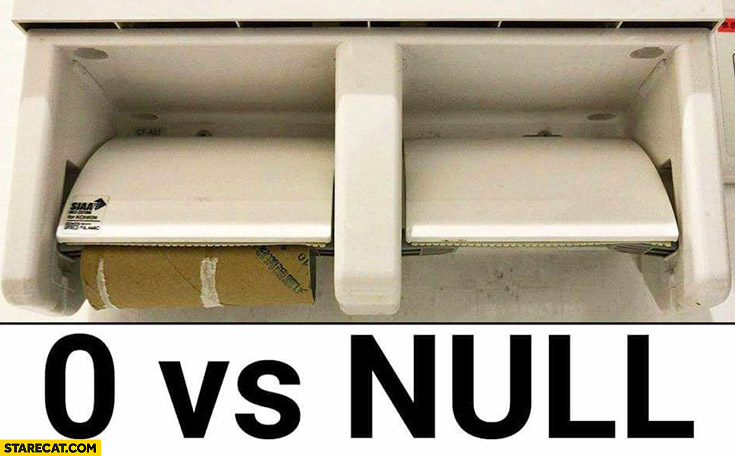
\includegraphics[width=0.4\textwidth]{null.jpg}
    \caption{}
\end{figure}
Verschil tussen IFNULL en ISNULL:
\begin{lstlisting}[language=SQL]
    IFNULL(expr1,expr2) -- is een controlestructuur en geeft expr2 terug als de waarde van expr1 NULL is.
    ISNULL(expr1) -- is een functie die controleert of expr1 al dan niet NULL is en dan 0 teruggeeft. In het andere geval wordt 1 teruggegeven. Dit kan handig gebruikt worden wanneer je een NULL wil omzetten naar 0 om bijvoorbeeld te kunnen sorteren.
\end{lstlisting}
\newpage
Voorbeelden:
\begin{lstlisting}[language=SQL]
-- (operator)
SELECT * 
FROM tblKlanten 
WHERE Ondernemingsnr IS NOT NULL       

-- (controlestructuur)
SELECT IFNULL(PrijsperEenheid,0) * 0.9 AS [Promotie]
FROM tblProducten 

-- (functie returnt een boolean)
SELECT * 
FROM tblorders
WHERE ISNULL(Leverdatum)
\end{lstlisting}

\subsubsection{Andere veel gebruikte functies}

\begin{lstlisting}[language=SQL]
-- cast
SELECT Naam, voornaam, CAST(Indienst AS date) FROM tblWerknemers

-- mathematische functies:
ABS
SIN
FIRST_VALUE
ENCRYPTBYKEY
CHOOSE
IIF(expr, true_value, false_value)  -- (returnt 1 van 2 waarden, afhankelijk van de boolean expression)
...
\end{lstlisting}


\subsection{GROUP BY}
Om te groeperen op basis van overeenkomsten tussen rijen

\begin{lstlisting}[language=SQL]
-- alle verschillende gemeenten tonen
SELECT Gemeente 
FROM tblKlanten 
GROUP BY Gemeente

-- alle gemeenten tonen met hun postnr, gesorteerd
SELECT Gemeente, Postnr
FROM tblklanten 
GROUP BY Gemeente, Postnr
ORDER BY Gemeente, Postnr -- beter overzicht door sortering
\end{lstlisting}

\subsubsection{Visuele voorstelling GROUP BY}

\begin{figure}[H]
    \centering
    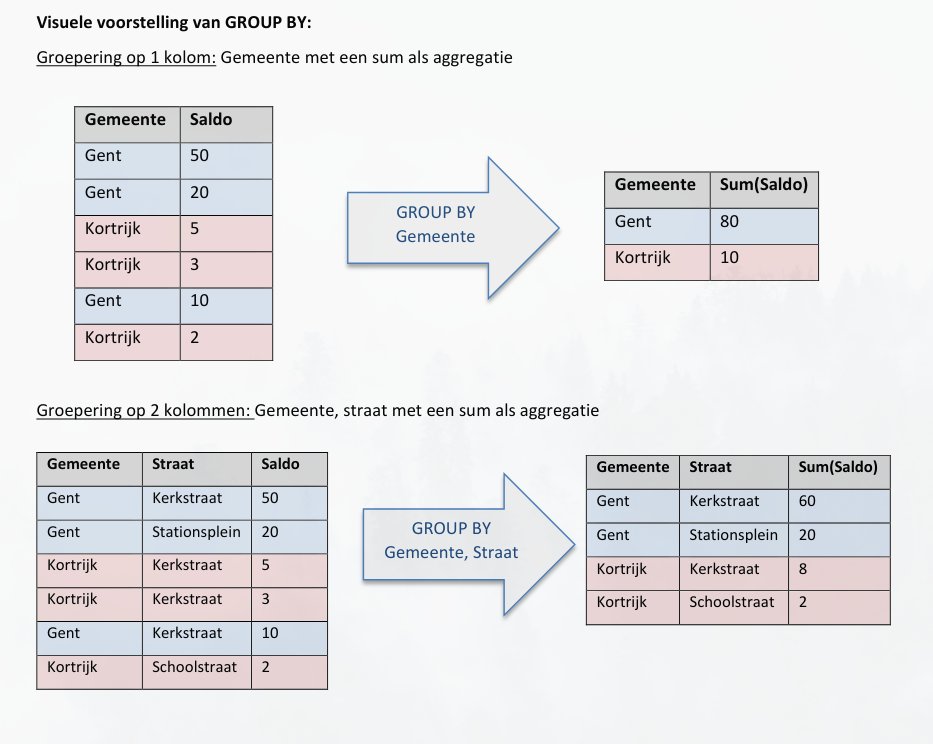
\includegraphics[width=0.8\textwidth]{Screenshot_20200219_154054.png}
    \caption{GROUP BY}
\end{figure}

\subsubsection{Belangrijk besluit}
Alle kolommen zonder een aggregatie functie (=zonder een berekening) moeten opgesomd worden in de  GROUP  BY  clause EN  in de  SELECT  clause.  Zoniet  krijg  je  foutief  gegroepeerde  data  (meestal  herkenbaar  omdat je maar één rij en dus te weinig data krijgt als resultaat).

\subsection{HAVING}
HAVING gebruiken wanneer je een aggregatiefunctie hebt in ORDER BY

\begin{lstlisting}[language=SQL]
GROUP BY  productnummer HAVING SUM(InBestelling)> 10

SELECT Gemeente, Postnr, sum  (Saldo) as saldo  
FROM tblklanten 
GROUP BY Gemeente,Postnr 
HAVING sum(Saldo) > 5000
ORDER BY  sum(Saldo) DESC
\end{lstlisting}

\begin{lstlisting}[language=SQL]
-- Dit werkt NIET:
WHERE SUM(InBestelling)> 10 GROUP BY productnummer
--  of
WHERE Productnummer>70 GROUP BY SUM(InBestelling) > 10

-- Dit werkt WEL:
GROUP BY productnummer HAVING SUM(InBestelling)> 10
-- of 
WHERE Productnummer>70 HAVING SUM(InBestelling)> 10
\end{lstlisting}

\subsection{controlestructuren in een SELECT statement}
\begin{itemize}
    \item IF()
    \item IFNULL()
    \item CASE
    \item 
\end{itemize}

\begin{lstlisting}[language=SQL]
SELECT CASE GESLACHT 
        WHEN '2' THEN 'Vrouw' 
        WHEN '1' THEN 'Man' ELSE '?' 
    END AS `Man/Vrouw`, 
    Familienaam 
FROM tblWerknemers
ORDER BY FIELD(`Man/Vrouw`,'Man','Vrouw','?'), Familienaam;
\end{lstlisting}

\section{SQL met meerdere tabellen}
\subsection{Primary Key \& Foreign Key}
Elk record in een tabel wordt geïdentificeerd door zijn enig en speciek nummer: de Primary Key (afgekort als PK). In de tblKlanten vinden we deze Primary Key [PK] terug in het klantnummer. 
De PK komt slechts één keer voor in deze tblKlanten.

Dezelfde waarde van de PK (klantnummer) komt terug in tblOrders. Omdat een klant meerdere orders kan hebben, vind je in tblOrders dit klantnummer meerdere keren terug.
Men spreekt dan over een Foreign Key (FK) in tblOrders. Wanneer men de PK en de FK verbindt, dan bekomt men een relatie.

\subsection{Relaties}

\begin{figure}[H]
    \centering
    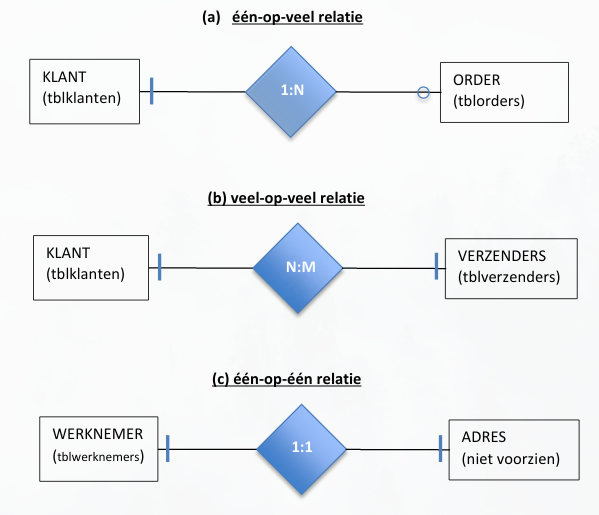
\includegraphics[width=0.6\textwidth]{Screenshot_20200226_143314.png}
    \caption{Verschillende soorten relaties}
\end{figure}

\begin{figure}[H]
    \centering
    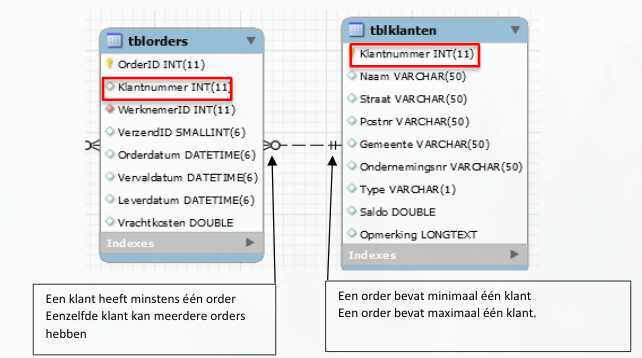
\includegraphics[width=0.6\textwidth]{Screenshot_20200226_144349.png}
    \caption{Tussen tblKlanten en tblOrders bestaat een 1:N relatie}
\end{figure}

\subsubsection{Relaties gebruiken in een query}
Het bevragen van 1 of meerdere gelinkte tabellen kan met T-SQL op 2 verschillende manieren gebeuren:

\begin{itemize}
    \item Via een SUBQUERY
    \begin{itemize}
        \item De WHERE of de FROM van de query krijgt zijn eigen query
    \end{itemize}
    \item Via een JOIN
    \begin{itemize}
        \item Er wordt gebruik gemaakt van de relatie (kan op verschillende manieren geinterpreteerd worden)
    \end{itemize}
\end{itemize}

\subsection{Joins}

JOIN is een manier om meerdere tabellen de combineren



\begin{itemize}
    \item Een OUTER JOIN haalt enkel de niet-gemeenschappelijke rijen eruit.  
    \item Een FULL OUTER JOIN combineert de INNER en OUTER JOIN en heeft de volledige verzameling van alle rijen weer.
    \item Een  LEFT  JOIN  haalt  alle  data  uit  de  linkse  tabel,  al  dan  niet  met  gemeenschappelijke  data  uit  de  rechtse  tabel. Met de term links verwijst men naar de tabelnaam die in FROM clausule staat.
    \item Een RIGHT JOIN haalt alle data uit de rechtse tabel, al dan niet met gemeenschappelijke data uit de linkse tabel.
\end{itemize}

Het gebruik van joins of subqueries laat niet alleen toe om gelinkte data te ondervragen (op basis van een ID) maar er kan ook onderzocht worden of er wel data bestaat (=zoeken op NULL).
Door het verbinden van verschillende tabellen kunnen naamverwarringen ontstaan. Oplossing $\Rightarrow$ gebruik sleutelwoord \bold{"AS"}

Bij ondervragingen op opzoekingen worden deze queries vaak uitgebreid met sleutelwoorden zoals:
\begin{itemize}
    \item ORDER BY
    \item DESC
    \item NOT IN
    \item BETWEEN
    \item LIKE
    \item AVG
    \item MAX
    \item HAVING
\end{itemize}

\begin{figure}[H]
    \centering
    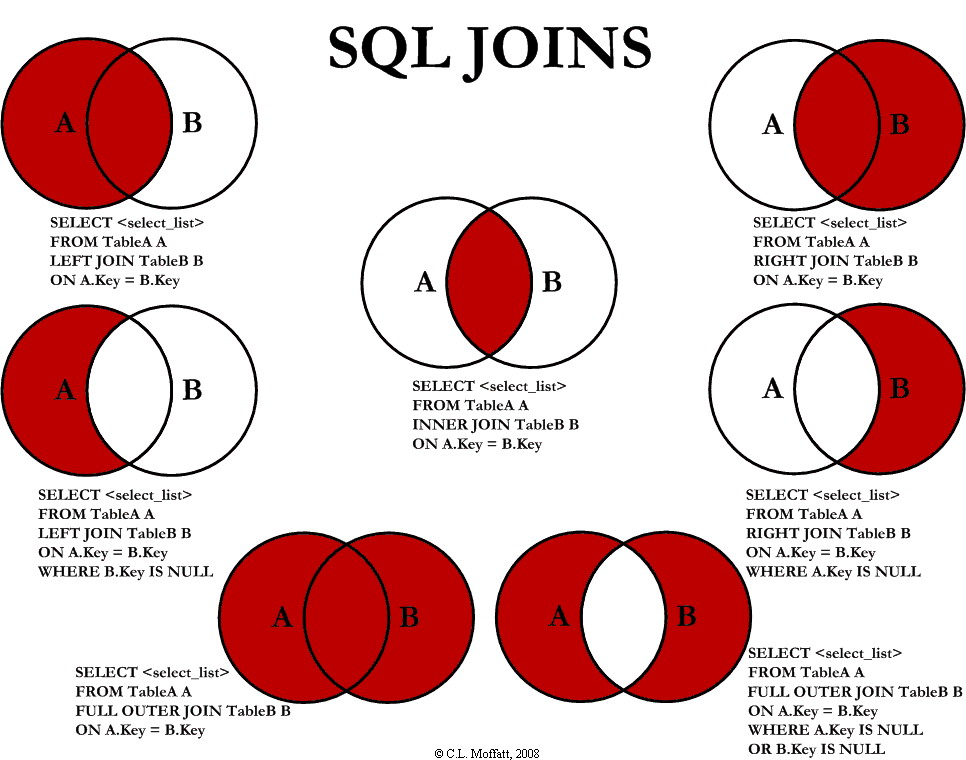
\includegraphics[width=\textwidth]{SQL Joins.jpg}
    \caption{Verschillende JOINS}
\end{figure}

\begin{lstlisting}[language=SQL]
-- cartesisch product = de kolommen worden gejoind door alle rijen cartesisch te combineren
-- Als tabelA 7 rijen heeft, en tabelB 6, dan is het resultaat van het cartesisch product 42 rijen (7*6):
SELECT *
FROM tblProducten, tblCategorieen 

-- Correcter:
SELECT *
FROM tblProducten, tblCategorieen
WHERE tblCategorieen.categorienummer = tblProducten.categorienummer

-- Met WHERE is dit niet zo overzichtelijk, we kunnen daarom ON gebruiken:
SELECT *
FROM tblProducten
JOIN tblCategorieen ON tblcategorieen.categorienummer = tblProducten.categorienummer

-- Voorbeeld met meer dan 2 tabellen:
SELECT  tblorders.*, tblklanten.*, tblwerknemers.* 
FROM tblklanten
JOIN tblorders ON tblklanten.klantnummer = tblorders.klantnummer
JOIN tblWerknemers ON tblorders.werknemerID = tblWerknemers.werknemerID

-- Gebruik aliasen met het sleutelwoord AS:
SELECT k.naam AS klantnaam, 
    w.familienaam as werknemernaam, 
    p.nederlandsenaam, 
    o.orderdatum as 'besteld op', 
    i.hoeveelheid AS aantal
FROM tblWerknemers AS w 
JOIN tblOrders AS o ON w.werknemerID = o.werknemerID 
JOIN tblKlanten AS k ON k.klantnummer = o.klantnummer
JOIN tblOrderinformatie AS i ON i. orderID = o.orderid
JOIN tblProducten AS p ON i.Productnummer = p.productnummer

-- Als de namen van de JOIN-kolommen gelijk zijn, kan de JOIN korter geschreven worden.
-- Je laat de JOIN-voorwaarde weg en voegt het woord NATURAL toe:
SELECT tblProducten.*, 
    tblCategorieen.categorienummer AS CategoryID
FROM tblProducten
NATURAL JOIN tblcategorieen
    
\end{lstlisting}

Een klassieke JOIN heeft altijd een kolom aan beide kanten van de relatie, maar soms kan het zijn dat 1 van die waardes niet is ingevuld (= NULL).
Soms moet je op zoek gaan naar deze nullen.

\underline{\bold{Bv}}: Welke producten werden nog nooit besteld?

\begin{figure}[H]
    \centering
    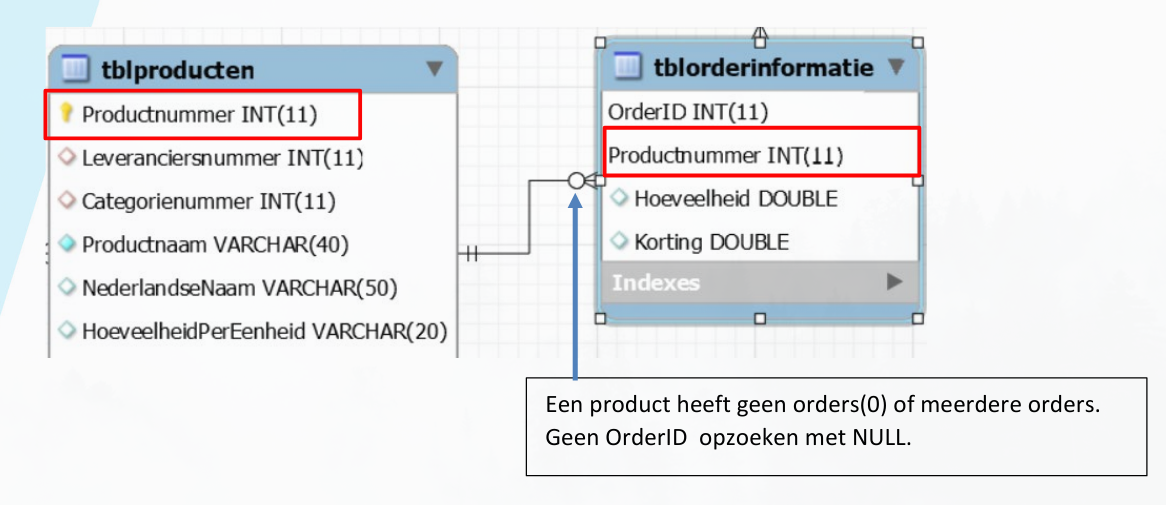
\includegraphics[width=0.7\textwidth]{Screenshot_20200304_151733.png}
    \caption{Het EER toont (zie de o) dat een product kan bestaan zonder order}
\end{figure}

Met een LEFT JOIN halen we deze producten op ook al zijn er geen gerelateerde orders:

\begin{lstlisting}[language=SQL]
SELECT p.productnummer as ProductNr, 
    p.nederlandsenaam AS Product, 
    o.orderid AS  bestelnummer, 
    o.hoeveelheid
FROM tblProducten AS p 
LEFT JOIN tblOrderinformatie AS o ON p.productnummer = o.productnummer
WHERE o.productnummer IS NULL;

-- we kunnen dit natuurlijk ook doen met een RIGHT JOIN, gewoon de omgekeerde operatie:
SELECT p.productnummer as ProductNr, 
    p.nederlandsenaam AS Product, 
    o.orderid AS  bestelnummer, 
    o.hoeveelheid
FROM tblOrderinformatie AS o -- deze keer tblOrderinformatie in de FROM-clause
RIGHT JOIN tblProducten AS p ON p.productnummer = o.productnummer -- en tblProducten in de JOIN-clause
WHERE o.productnummer IS NULL;

-- Voorbeeld: Welke werknemers hebben nog nooit een bestelling geplaatst? 
SELECT o.orderid, w.werknemerid, w.familienaam, w.functie 
FROM tblOrderso
RIGHT JOIN tblWerknemers w on o.werknemerid = w.werknemerid
WHERE o.orderid IS  NULL
\end{lstlisting}

\subsubsection{Speciale JOINS}

\bold{CROSS JOIN}
\begin{itemize}
    \item = JOIN die zonder voorwaarde het \underline{cartesisch product} aanmaakt van alle kolommen in beide tabellen
    \item Als je alle kolommen van tabelA wil 'kruisen' met alle kolommen van tabelB
\end{itemize}
\bold{UNION}
\begin{itemize}
    \item Om tabellen samen te voegen, die dezelfde structuur hebben
    \item Aantal velden en datatypes moeten perfect kloppen 
    \item = Doet automatisch een DISTINCT-operatie, tenzij je UNION ALL gebruikt.
    \item Typische UNION toepassing: je wil jouw eigen tabel (vb adressen) uitbereiden met de tabeldata van een collega (vb addressen van jouw collega)
\end{itemize}

\subsection{Subqueries}
\subsubsection{Voorbeeld op subqueries}

Toon alle klanten die in een gemeente zijn gevestigd waar ook een werknemer woont. 

Zonder te weten hoe een join werkt, kunnen we dit al uitvoeren met 2 afzonderlijke queries:

\begin{itemize}
    \item Een query met een lijst van alle gemeentes waar een werknemer woont
    \item Een query met een lijst van alle klanten die in deze gemeenten wonen.
\end{itemize} 

Rest nog om beide queries te combineren, waarbij de WHERE een subquery krijgt:


\begin{figure}[H]
    \centering
    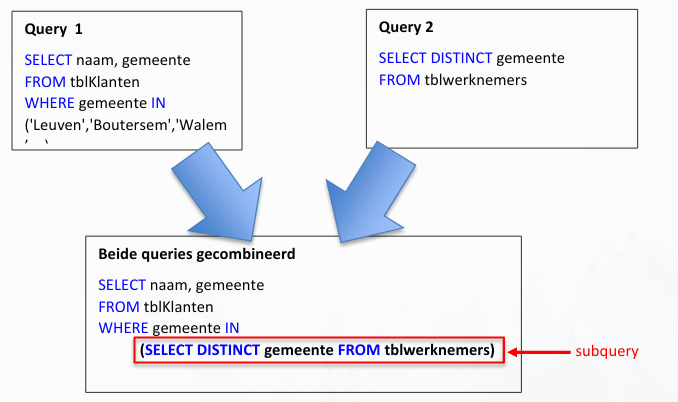
\includegraphics[width=0.8\textwidth]{Screenshot_20200226_153136.png}
    \caption{Voorbeeld subquery}
\end{figure}

Een subquery komt altijd tussen haakjes voorafgegaan door een andere aanroepende tabelexpressie. 
Het keywoord in de aanroepende query is meestal IN of NOT IN of WHERE EXISTS of WHERE NOT EXISTS maar kan ook eenvoudige weg WHERE zijn:

\begin{lstlisting}[language=SQL]
-- Voorbeeld: Productnaam van het duurste product
SELECT productnummer, productnaam 
FROM tblProducten 
WHERE PrijsPerEenheid =(
    SELECT max(PrijsPerEenheid)  
    FROM tblproducten 
)

-- Voorbeeld: Alle klanten die geen orders hebben geplaatst (klanten die niet te vinden zijn in tblOrders)
SELECT Naam 
FROM tblklanten 
WHERE NOT EXISTS (
    SELECT * 
    FROM tblOrders 
    WHERE tblOrders.Klantnummer = tblklanten.Klantnummer
) 

-- Voorbeeld: Dezelfde gemeente en postcode in een andere tabel ophalen 
SELECT * 
FROM tblwerknemers
WHERE (gemeente, postcode) in  (
    SELECT plaats,postcode 
    FROM tblleveranciers
)

-- meerdere subqueries zijn mogelijk:
... WHERE waardeX BETWEEN (subquery_1) AND (subquery_2)

\end{lstlisting}


\section{Data aanpassen met UPDATE}

\begin{lstlisting}[language=SQL]
UPDATE tbLKlanten
SET Postnr = '3021'
WHERE Gemeente = 'Herent' -- NOOIT DE WHERE VERGETEN: anders zet je alle postcodes op 3021!
\end{lstlisting}

\subsection{UPDATE volgens een filter in dezelfde tabel}

\begin{lstlisting}[language=SQL]
-- Voorbeeld: 
SELECT Vervaldatum, 
    DATE_ADD(Vervaldatum,INTERVAL 7 DAY) AS `Latere Vervaldatum`, 
    Vrachtkosten, 
    Vrachtkosten * 1.1 AS 'Verhoogde Vrachtkosten'
FROM tblOrders
ORDER BY Vervaldatum DESC
\end{lstlisting}

\begin{figure}[H]
    \centering
    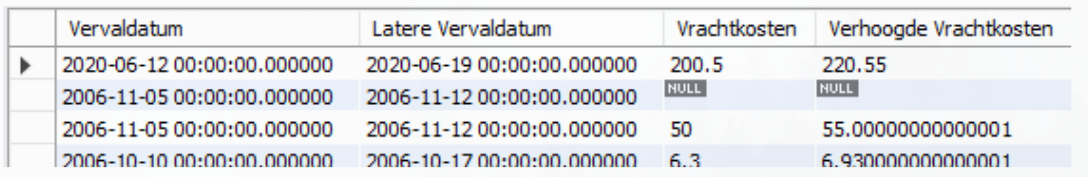
\includegraphics[width=0.7\textwidth]{Screenshot_20200304_154106.png}
    \caption{Output bovenstaande SELECT-query}
\end{figure}

\begin{lstlisting}[language=SQL]
-- Wijzig nu de vrachtkosten en verhoog ze met 10%, de vervaldatum mag 7 dagen later worden. 
-- Recente vervaldata vooraan vermelden!

UPDATE tblOrders as o
SET Vervaldatum = DATE_ADD(Vervaldatum, INTERVAL 7 DAY),
Vrachtkosten = Vrachtkosten * 1.1

\end{lstlisting} 

\subsection{Updates volgens een filter in een gerelateerde tabel}
Soms wil je een update doen waarvan de voorwaarde (wat je wil wijzigen) in een andere gerelateerde tabel moet gezocht worden. 
Dit betekent dat we de voorwaarde moeten zoeken in deze andere tabel met behulp van JOINS of SUBQUERIES. 
De tabelnaam wordt bijvoorbeeld gevolgd door een JOIN statement:

\begin{lstlisting}[language=SQL]
UPDATE tblproducten as P 
JOIN tbl categorieen as C on C.productnummer = P.productnummer 
SET UitAssortiment = 1
WHERE . . . . .     
\end{lstlisting}

\section{Data verwijderen met DELETE}
\subsection{Syntax}

\begin{lstlisting}[language=SQL]
DELETE FROM tabel
WHERE x = waarde
\end{lstlisting}

\bold{Opmerking:} Het volledig deleten van records is iets waar heel voorzichtig mee omgegaan wordt in de industrie.
Eerder zal men de niet-langer-nodige records verplaatsen naar een backup-tabel.

\subsection{Delete van records en relaties}
Als er een 1-op-veel relatie is tussen 2 tabellen kan bij het verwijderen van een record aan de 1-zijde worden uitgevoerd aan de veel-zijde van de relatie.
Wat in de gerelateerde tabel al dan niet verwijderd wordt, hangt af van de definitie van de relatie.

Dit verwijder gedrag kan ingesteld worden voor \underline{\bold{4 types}}:

\begin{enumerate}
    \item \bold{Restrict}:
    \begin{itemize}
        \item Alle mogelijke delete acties op de parent verhinderd wanneer er nog gerelateerde records bestaan in de child tabel
        \item Dit is het default type by MySQL
    \end{itemize}
    \item \bold{Cascade}:
    \begin{itemize}
        \item Alle gerelateerde records worden ook verwijderd
        \item Afgeraden want kan leiden tot ongewenst dataverlies
        \item \underline{Voorbeeld:} bij het verwijderen van een categorie in tblCategorie, worden alle producten uit deze categorie in tblProducten ook verwijderd.:
    \end{itemize}
    \item \bold{Set Null}:
    \begin{itemize}
        \item Bij het verwijderen van een record uit een parenttabel, worden de gerelateerde \underline{keyvelden} op NULL gezet.
        \item Zo wordt het record in de parenttabel wel verwijderd, maar in de childtabel worden de gerelateerde Foreign Keys op NULL gezet.
        \item De data van de andere velden in het gerelateerde record blijft ongewijzigd
        \item \underline{Voorbeeld:} Bij het verwijderen van een categorie in tblCategorie, krijgen de gerelateerde producten in tblProducten een NULL-waarde voor het veld 'categorienummer'
    \end{itemize}
    \item \bold{No Action}:
    \begin{itemize}
        \item Met 'No Action' kan een parent record niet verwijderd worden als er nog kinderen zijn.
        \item No Action en Restrict hebben in MySQL hetzelfde resultaat
        \item T-SQL beschrijft een klein verschil tussen beide
        \begin{itemize}
            \item RESTRICT is harder en staat geen enkele wijziging toe op parent of child.
            \item Bij No Action wordt de expressie wel getest en kan de child tabel ongewijzigd worden gelaten indien mogelijk volgens de relatie 
        \end{itemize}
    \end{itemize}
\end{enumerate}

De standaard T-SQL bschikt nog over een extra keywoord: SET DEFAULT. 
Bij een delete van een parent, worden de kinderen ingesteld op hun default waarde. 
Het keywoord ‘SET DEFAULT’ bestaat niet in MySQL.

Welke type er gebruikt wordt voor een relatie in de database, kan je in MySQL workbench terugvinden:
de database $\Rightarrow$ design $\Rightarrow$ “Foreign Keys” tabblad

\subsection{Voorbeeld: DELETE types toegepast}
\begin{lstlisting}[language=SQL]
-- we willen het categorie nummer 17 verwijderen uit tblcategorieen:
SELECT * FROM artemis.tblproducten WHERE Categorienummer = 17;
\end{lstlisting}

\begin{figure}[H]
    \centering
    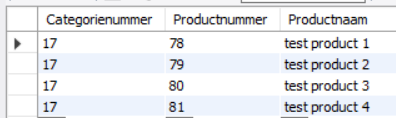
\includegraphics[width=0.6\textwidth]{7-3.png}
    \caption{Output bovenstaande SELECT-query}
\end{figure}

We bekijken de manieren om deze categorie te DELETEN op basis van op welk DELETE type de relatie staat:

\subsubsection{Met RESTRICT en NO ACTION}
\begin{lstlisting}[language=SQL]
-- we moeten eerst alle producten met categorienummer 17 verwijderen, anders krijgen we een error:
DELETE FROM producten WHERE categorienummer = 17 ;
-- dan de categorie zelf
DELETE FROM tblcategorieen WHERE categorienummer = 17
\end{lstlisting}

\subsubsection{Met SET NULL}
\begin{lstlisting}[language=SQL]
DELETE FROM tblcategorieen
WHERE categorienummer = 17
-- Categorie 17 is verwijderd uit tblcategorieen. 
-- In de tblproducten is categorienummer 17 aangepast naar NULL bij elk product van categorie 17.
\end{lstlisting}

\subsubsection{Met CASCADE}
Zelfde operatie als bij SET NULL, maar deze keer zijn alle producten van categorie 17 verwijderd.

\subsection{DELETE en JOINS}
Het komt vaak voor dat je een DELETE wil uitvoeren waarbij een voorwaarde in een andere gerelateerde tabel nodig is. 
Men noemt dit ook een \bold{MULTI-DELETE}. Dit kan worden uitgewerkt met een JOIN of een subquery.

\subsubsection{Met een JOIN}
\underline{Voorbeeld:} 

We willen details van een order verwijderen (tblOrderinformatie) maar kennen alleen de leverdatum (tblOrders)
\begin{lstlisting}[language=SQL]
DELETE tblorderinformatie
FROM tblorderinformatie
JOIN tblOrders as O on O.OrderId = tblorderinformatie.OrderID
WHERE O.leverdatum = "2006-05-15"
\end{lstlisting}


\subsubsection{Met een subquery}

\underline{Voorbeeld:} Een order verwijderen waarvan de werknemer naam in een andere tabel staat.
\begin{lstlisting}[language=SQL]
DELETE tblorders
FROM tblORDERS
WHERE werknemerID IN (
    SELECT DISTINCT werknemerid 
    FROM tblwerknemers
    WHERE familienaam ="Peeters"
)
\end{lstlisting}

\section{Gegevens invoeren met INSERT}
Je kan op een aantal manieren gegevens toevoegen aan je databank:

\begin{itemize}
    \item 1 nieuw record toevoegen
    \item Meerdere records toevoegen uit andere tabel
    \item Nieuwe tabel op basis van een andere tabel
\end{itemize}


\subsection{Nieuw record invoeren}
\begin{lstlisting}[language=SQL]
INSERT INTO tblWerknemers (Familienaam, Voornaam)
VALUES ('Vannieuwenhuyse','Johan')
\end{lstlisting}
De volgorde van de velden die je opgeeft en de datatypes ervan moet gelijk zijn.

Je dient wel te weten of de Primary Key van deze tabel aangemaakt wordt door het systeem 
(= automnummering = autoidentity = autoincrement = AI ) of indien je zelf een uniek nummer wil opgeven.
Dit kan je vinden in de tabel design modus in MySQL Workbench

Vermeld je geen veldnamen in de INTO dan word je verondersteld om alle waarden in te vullen bij Values. 
Die waarden kunnen ook NULL zijn. Deze NULL is bijvoorbeeld nodig voor een Primary Key van het AutoIncrement.

\begin{lstlisting}[language=SQL]
INSERT INTO tblCategorieen
VALUES (NULL, "BBQ" , "BBQ vlees");
\end{lstlisting}

\subsubsection{Problemen bij INSERT}
\begin{itemize}
    \item Voer je een waarde in die te veel karakters heeft zoals toegelaten door een kolom, dan krijg je een truncate error
    \item Ook verkeerde datatypes worden niet geaccepteerd
    \item Manueel een zelfde primary key nogmaals invullen kan niet
    \item Let op de volgorde van de kolommen.
\end{itemize}

\subsection{Gegevens toevoegen uit een andere tabel}
Met een subquery: 
\begin{lstlisting}[language=SQL]
INSERT INTO tblwerknemers(`Familienaam`, `Adres`, `Gemeente`, `Postcode`)
    SELECT naam,straat, gemeente, postnr
    FROM tblKlanten
    WHERE gemeente= 'Herent'
\end{lstlisting}

\subsection{Nieuwe tabel op basis van een andere tabel}

\begin{lstlisting}[language=SQL]
CREATE TABLE tblParticulieren
    SELECT *
    FROM tblKlanten
    WHERE type= 'p'
\end{lstlisting}

\subsubsection{Backup maken}
\begin{lstlisting}[language=SQL]
CREATE TABLE 2019_tblKanten_bak
    SELECT *
    FROM tblKlanten
    blKlanten
\end{lstlisting}

\subsection{Nieuwe waarden toevoegen en relaties.}
Waarden toevoegen in een tabel kan je niet als de foreign keys van deze tabel nog niet gekend zijn als primary keys in de parent tabellen.

\underline{Voorbeeld:}
Je kan geen producten toekennen aan categorienummer 55, als je niet eerst dit categorienummer aanmaakt in tblcategorieën.
\begin{lstlisting}[language=SQL]
INSERT INTO tblproducten (Leveranciersnummer,Categorienummer,Productnaam, BTWCode , UitAssortiment)
VALUES (12, 55 , 'Nieuw product', 3, false);
\end{lstlisting}

\section{Views}
Views bevatten een aantal instructies of formules, gebaseerd op bestaande tabellen om nieuwe “virtuele”
tabellen samen te stellen en vervolgens daarop queries uit te voeren.

\begin{lstlisting}[language=SQL]
CREATE VIEW `vwProducten` AS
    SELECT tblProducten.*, 
        tblCategorieen.categorienummer as cNr, 
        tblCategorieen.categorienaam
    FROM tblProducten
    JOIN tblCategorieen ON tblProducten.categorienummer = tblCategorieen.categorienummer
\end{lstlisting}

Eenmaal aangemaakt kunnen views ondervraagd worden met standaard queries 
en met gebruik van de kolomnamen van de view.

\subsection{Wanneer views gebruiken?}
\begin{itemize}
    \item Veelvuldig hergebruik van dezelfde query: maak in de plaats een simpele view aan.
    \item Het herorganiseren van een tabel: aanpassen van kolomnamen. 
    \item Combineren van views door verschillende views te gebruiken in subqueries $\Rightarrow$ verhoogt de leesbaarheid.
    \item Extra beschikbare opties bij een view kunnen security en integriteit bevorderen.
\end{itemize}

\section{Python in Datamanagment}
\subsection{Data-accessor (DA)}
\begin{itemize}
    \item Een data-accessor zorgt voor de toegang tot een database
    \item Data-accessor code wordt vaak toegeleverd door de \bold{databaseprovider} 
    \item MySQL: C\# en Python
    \item Redis: Javascript
    \item MSSQL: Python
    \item JSON: Javascript
\end{itemize}

\subsubsection{De onderdelen van een data-accessor}
\begin{enumerate}
    \item Een connectionstring 
    \item Software voor het uitvoeren van CRUD-acties
    \item Een \bold{repository} met SQL-expressies voor die CRUD-acties
\end{enumerate}

\subsubsection{Hoe zien de onderdelen van een DA eruit?}
Elk deel van de DA krijgt zijn eigen file: \textit{Single Responsibility Principle}

\begin{figure}[H]
    \centering
    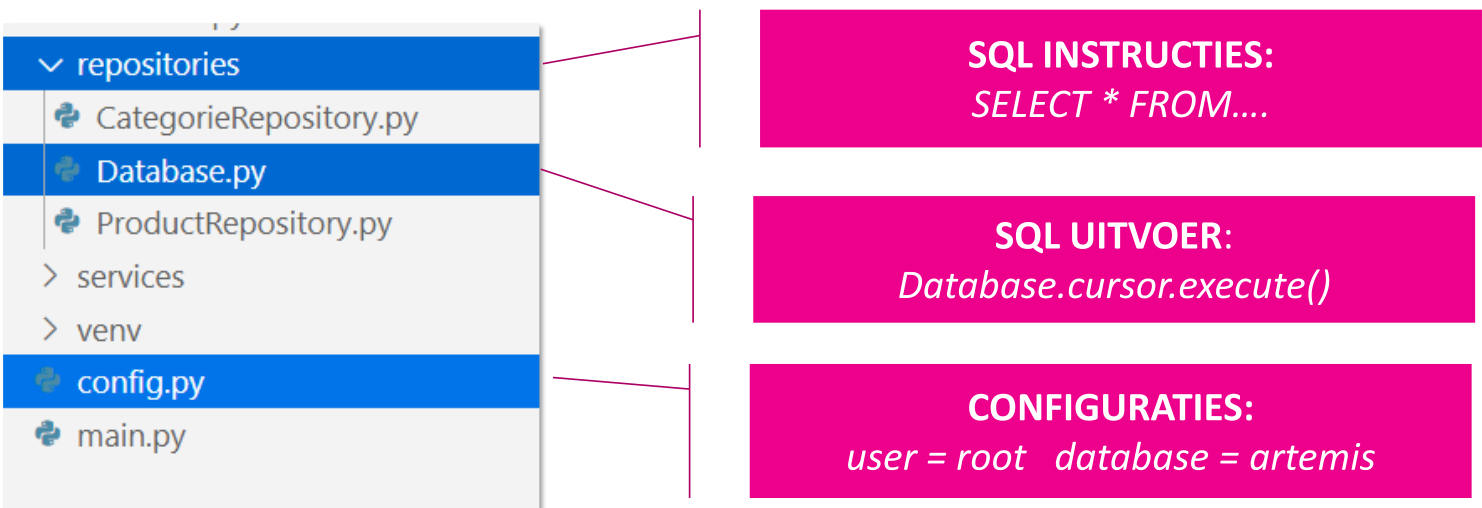
\includegraphics[width=0.7\textwidth]{Screenshot_20200503_152141.png}
    \caption{Single Responsibility principle}
\end{figure}

\subsubsection{config.py}
Bevat ALLE configuraties die “hardcoded” ingebracht worden in onze toepassing $\Rightarrow$ Inhoud aanpassen voor jouw MySQL Server of MariaDB instantie.

\begin{lstlisting}
[connector_python]
user = root
host = 127.0.0.1
port = 3306
password = root
database = artemis

[application_config]
driver = 'SQL Server'
\end{lstlisting}

\subsubsection{Database.py}
Bevat TWEE TYPES om code op de database server uit te voeren:
\begin{itemize}
    \item Database.cursor.fetch() : enkel om data te lezen op MySQL (Read)
    \item Database.cursor.execute(): voor het wijzigen van data (Create-Update-Delete)
\end{itemize}

Database.\_\_open\_connection() gebruikt config.py.

\begin{figure}[H]
    \centering
    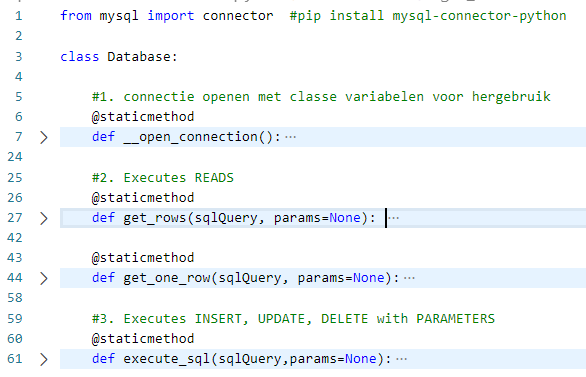
\includegraphics[width=0.6\textwidth]{database-py.png}
    \caption{Database.py}
\end{figure}

\subsubsection{Repository.py}
\begin{itemize}
    \item Database.py blijft dezelfde voor elke applicatie.
    \item Het repository bevat ALTIJD de SQL-expressies (CRUD).
    \item Maar: De implementatie van een repository kan wel verschillen naargelang de toepassing (fullstack != datamanagement):
    \begin{itemize}
        \item Repository fullstack: JSON API op de Raspberry PI met MariaDB
        \item Repository Datamanagement: Console applicatie op de PC met MySQL
    \end{itemize}
\end{itemize}

\subsubsection{Aandachtspunten voor een data-accessor}
\begin{itemize}
    \item Een DA moet functioneel perfect werken (=data ophalen).
    \item Een DA mag de applicatie niet laten crashen en daarom:
    \begin{itemize}
        \item Een DA valideert de input gegevens van een gebruiker en informeert deze over foutieve ingave.
        \item Een DA beschermt de toepassing tegen moedwillig kwaad opzet door het invoeren van script(virus) of onbestaande data.
    \end{itemize}
\end{itemize}


\subsection{Repository in Fullstack}
Kan eenvoudig gehouden worden voor de API:
\begin{itemize}
    \item Er is slechts één repository.
    \item Er worden geen modellen aangemaakt.
\end{itemize}

Meer info in labo fullstack

\subsection{Repository in Datamanagement}
Er is een verband tussen de database tabellen op de server en de classes in OOP

\begin{itemize}
    \item Maak voor elke SQL tabel een Python class (=MODEL)
    \item Maak voor elke kolom in de tabel een property in de class.
\end{itemize}

\subsubsection{Het repository en zijn model}
Het model (de Python-klasse) wordt gebruikt in een repository (Repository.py), die toegang geeft tot de MySQL databank.

Bij elke functie in het repo komt steeds hetzelfde patroon terug:
\begin{enumerate}
    \item VALIDEER de user input.
    \item De SQL expressie met parameters. Parameter = must = verhindert SQL injectie
    \item Controleer de return vanuit Database.cs:
    \begin{itemize}
        \item Ofwel een bevestiging van de geslaagde actie.
        \item Ofwel een NONE die een ERROR aanduidt.
    \end{itemize}
    \item Return het Database.cs resultaat
\end{enumerate}

\subsubsection{De object mapper}
De python functie map\_to\_object(row) zet elke rij om naar een object van het model.

\subsection{Hoe de repo gebruiken in je toepassing}
Een REPO DOET ENKEL aan datamanagement (CRUD) en niets anders.

Wie het repo gebruikt noemen we een SERVICE. De service print de database resultaten.


\section{Database Management Systemen (DBMS)}
\subsection{Een DBMS kiezen}
Een \bold{database} is alles wat data verzamelt en organiseert.
Dit kan op verschillende formaten of op verschillende plaatsen met verschillende apperatuur.
Wanneer je een database wenst te maken, verplicht dit ons om keuze te maken tussen de beschikbare database structuren:

\begin{itemize}
    \item Single-user of multi-user databases
    \item Gestructureerde (MSSQL) of niet-gestructureerde (NoSQL, Excel) data bijhouden
    \begin{itemize}
        \item Soms wel relationele of niet-relationele databases genoemd
        \item Met 'gestructureerd' verwijst men naar data opgeslagen in verschillende zelf beschrijvende en samenhangende tabellen
    \end{itemize}
    \item Via eenvoudige tekstbestanden 
    \begin{itemize}
        \item zoals *.csv
        \item Meestal voor kleinere configuratiebestanden
    \end{itemize}
    \item Hierarchische structuren
    \begin{itemize}
        \item zoals *.xml
    \end{itemize}
    \item Geserializeerde objecten
    \begin{itemize}
        \item zoals *.json
        \item Serialisatie zorgt dat een object omgezet wordt naar een transporteerbaar formaat zoals een tekst string.
    \end{itemize}
    \item Gecentraliseerd
    \begin{itemize}
        \item de data komt op één specifieke server, of gedistribueerd, waarbij de data over verschillende servers van een netwerk verspreid wordt.
    \end{itemize}
    \item Installatie lokaal, 
    \begin{itemize}
        \item op eigen database-server(s) of via internet op een (te betalen) Cloud systeem
        \item zoals Amazon Web Services, Microsoft One Drive, Google Cloud , Alibaba cloud , IBM cloud
    \end{itemize}
\end{itemize}

Elk formaat of type installatie heeft voordelen en nadelen

\subsection{Elementen in een database toegang}

\begin{enumerate}
    \item Gebruikers
    \begin{itemize}
        \item Worden onderverdeeld in rollen: admin, superuser, read-only user, testuser, \dots
        \item Hebben specifieke eigenschappen (naam, email, taal, \dots)
    \end{itemize}
    \item De database toepassing (of database applicatie) 
    \begin{itemize}
        \item = een set van computerprogramma's die data aanbiedt aan de users en toelaat deze data te lezen of wijzigen via statements en instructies
        \item Een applicatieprogramma kan in verschillende talen geschreven worden voor verschillende types users.
    \end{itemize} 
    \item Het DBMS (Database Management Systeem)
    \begin{itemize}
        \item Is een computerprogramma dat toelaat de werkelijke data van de database te lezen, wijzigen of administreren
        \item \underline{Voorbeelden:} Microsoft SQL Server, Oracle Corporation's MySQL, key-value store RocksDB van Facebook, de NoSQL App Engine Datastore van Google, \dots
    \end{itemize}
    \item De database
    \begin{itemize}
        \item Is een collectie van data verzameld in verwante tabellen of andere structuren.
        \item wordt geïnstalleerd op één of meerdere database servers,
    \end{itemize}
\end{enumerate}

\subsection{RDBMS overzicht}
\begin{itemize}
    \item = Relational Database Management System
    \item Verwijst naar een zelf beschrijvende verzameling van verwante tabellen
\end{itemize}

\bold{Self-describing:}
\begin{itemize}
    \item Geen extra uitleg nodig om de tabel structuur te begrijpen
    \item de metadata is genoeg (= namen van tabellen, rijen, definities en eigenschappen)
\end{itemize}

\bold{Related tabels}
\begin{itemize}
    \item De tabellen zijn verwant met elkaar (= gerelationeerde tabellen). 
    \item De verwantschap tussen tabellen wordt het best en duidelijk weergegeven in een databasemodel of ERD (Entiteit Relatie Diagramma).
\end{itemize}


De meest gebruikte relationele databases vermelden we MSAccess, MSSQL en MySQL, maar ook Oracle en DB2 voorzien relationele databases. Wij gebruiken vooral MySQL.
De techniek tot correct gebruik en aanmaken van RDBMS-databases is bij elk van deze dezelfde. \bold{Syntax en datatypes kunnen wel afwijken!}.

\begin{itemize}
    \item MS Access:
    \begin{itemize}
        \item Maakt deel uit van MS Office.
        \item File georiënteerd (file type *.mdb)
        \item Voldoende om een driver te installeren om de gegevens te bevragen
        \item Handig om snel een database toepassing op te zetten door formulieren en rapporten te integreren in de ontwikkelomgeving
    \end{itemize}
    \item MSSQL:
    \begin{itemize}
        \item Server oplossing van Microsoft met verschillende subversies (nu 5), die vaak vernieuwd worden
    \end{itemize}
    \item SQLite
    \begin{itemize}
        \item Heeft geen afzonderlijk server process en gebruikt een in process library om plain files op disk te schrijven.
        \item Niet geschikt voor meerdere concurrent users of voor veel concurrent database operaties.
        \item Veel gebruikt in devices (Android iOS – televisies, wagens) en in diverse applicaties (Skype, iTunes, Dropbox)
        \item Weinig setup nodig
    \end{itemize}
    \item PostgreSQL
    \begin{itemize}
        \item Opensource database met vooral veel features en een sterk datasupport (inclusief JSON) voor vele talen
        \item Volgt sterk de ANSI-SQL standaard
    \end{itemize}
    \item Oracle
    \begin{itemize}
        \item Is een populaire maar closed-source met een dure licentie.
        \item Stabiel, zeer uitgebreide feature set
    \end{itemize}
\end{itemize}

Een volledige lijst van RDBMS vind je op \url{
    https://en.wikipedia.org/wiki/List\_of\_relational\_database\_management\_systems
    }

\section{Ontwerpen van een RDBMS}
Het opbouwen van een database kan naargelang het type op verschillende manieren gebeuren. Een NoSQL
database ontwerp je niet ( en gebruik je ook niet) op dezelfde manier als een relationele database zoals MSSQL
of MySQL.

Het ontwerpen van een relationele (!) database delen we op in de volgend drie grote stappen:
\begin{enumerate}
    \item De voorstudie (=klantprobleem)
    \item Het entiteit relatie diagramma (ERD) of database model aanmaken(=klant akkoord)
    \item Ontwerp van tabellen en relaties (=ontwikkelaar niveau)
\end{enumerate}

\section{De voorstudie}

De voorstudie (ook analyse genoemd) kan vertrekken vanuit verschillende standpunten (= kan vertrekken vanuit
een ander type klant):

\begin{enumerate}
    \item \bold{Op basis van bestaande gegevens:}
    \underline{Voorbeeld:} de data bijgehouden door een secretaresse wordt te complex, waardoor fouten binnensluipen
    in de verschillende tabbladen van een spreadsheet.
    \item \bold{Een volledig nieuw databasesysteem ontwikkelen:} Hiertoe moet een grondig onderzoek gebeuren wat de
    eisen zijn van de applicatie (en zijn gebruikers) om van daaruit de database te ontwerpen.
    \underline{Voorbeelden:} Installatie van een ERP (Enterprise Resource Planning) of CRM (Customer Relationship
    Management) pakket in een firma.
    \item \bold{Herontwerpen van een bestaande database:} Vaak gebruikt men hier het woord migratie, wat zowel duidt
    op het combineren van verschillende bestaande databases tot het upgraden ervan met extra data.
    \underline{Voorbeeld:} de firma start met een nieuw krachtiger programma omwille van performantie redenen.
\end{enumerate}

\section{Het model en zijn Entiteit Relatie Diagram (ERD)}

Vanuit de analyse van data (= de voorstudie) wordt een entiteit relatie model opgesteld. 
Dit ER-Model (=database model) bewijst vooral zijn belang bij het maken van afspraken met opdrachtgevers
en het vastleggen van constraints (beperkingen op de data en zijn relaties).Het Entity Relation Diagram (ERD) is de weergave van dit entiteit relatie model. 

\subsection{Entiteit}
Een \bold{entiteit} is elk identificeerbaar ding (instantie), een identificeerbaar iets met gegevens
\begin{itemize}
    \item heeft unieke kolommen of eigenschappen. Men spreekt over \bold{attributen}.
    \item heeft \bold{unieke rijen} (geen dubbele data)
\end{itemize}

\subsubsection{Eigenschappen:}
\begin{itemize}
    \item Entiteiten kunnen functioneel afhankelijk zijn van elkaar (= hebben een relatie).
    \item De \bold{determinant} is het attribuut dat eenduidig de entiteit bepaalt en gebruikt wordt om de afhankelijkheid te realiseren. 
    \item Er kunnen meerdere attributen nodig zijn voor één determinant (=samengestelde determinant).
    \item \underline{Voorbeeld: }
    \begin{itemize}
        \item (Naam, Voornaam) $\rightarrow$ (Haarkleur, lengte, schoenmaat, gewicht)
        \item Dit wil zeggen: als je de naam en voornaam weet in een tabel, dan weet je ook haarkleur, lengte, schoenmaat en gewicht
    \end{itemize}
\end{itemize}

\subsubsection{Sterke entiteiten:}
\begin{itemize}
    \item Kan op zichzelf bestaan
    \item In een diagramma: een rechthoek met vierkante hoeken
    \item \underline{Voorbeelden:} 
    \begin{itemize}
        \item een onderzoek met zijn resultaten
        \item een gebouw met de gegevens over infrastructuur en aantal verdiepingen
    \end{itemize}
\end{itemize}

\subsubsection{Zwakke entiteiten:}
\begin{itemize}
    \item Onderdeel van een andere entiteit
    \item Op zich onvoldoende om te bepalen over welke parent het gaat
    \item In een diagramma: een rechtzoek met ronde hoeken
    \item \underline{Voorbeelden:}
    \begin{itemize}
        \item patiënt als zwakke entiteit van een onderzoek
        \item appartement nummer als zwakke entiteit van een gebouw
    \end{itemize}
\end{itemize}

De \bold{determinant} staat in het vet:

\begin{figure}[H]
    \centering
    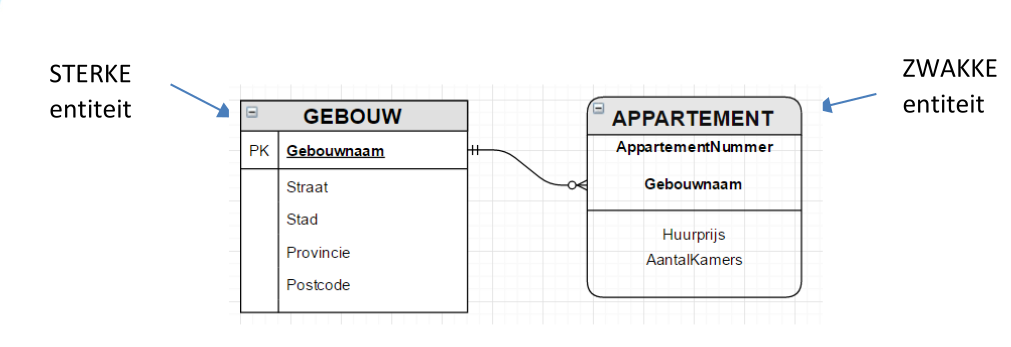
\includegraphics[width=0.8\textwidth]{Screenshot_20200318_144749.png}
    \caption{Sterke en zwakke entiteit}
\end{figure}

\subsection{Sleutels}

\subsubsection{Primary Key (PK)}

\begin{itemize}
    \item De \bold{unieke} determinant voor elke rij van gegevens: identificeert de volledige entiteit
    \item Kan al dan niet samengesteld zijn
    \item De verzameling van alle mogelijke unieke determinanten (inclusief de PK) noemt men “kandidaat keys”; waarbij de PK deze is die uiteindelijk gekozen werd voor het ontwerp.    
\end{itemize}

\subsubsection{Surrogaatsleutel / identity key}
\begin{itemize}
    \item Men kan het ook overlaten aan het databasesysteem om zelf deze unieke keys [PK] voor de entiteiten aan te maken, dan noemen we deze sleutel een surrogaatsleutel
    \item Numeriek (een integer) waarvan je zelf beslist hoe groot de increment (=hoeveel de integer vermeerderd wordt bij een nieuwe rij gegevens)
\end{itemize}

\subsubsection{Minimale sleutel}
\begin{itemize}
    \item Het kan dat meerdere attributen (eigenschappen) moeten gebruikt worden voor het bekomen van een unieke key
    \item Men spreekt in dit geval van een minimale sleutel, waarbij elk element noodzakelijk is voor het bekomen van de unieke key
    \item Dus altijd een samengestelde key: heeft meerdere attributen
\end{itemize}

\subsubsection{Alternatieve sleutel (AK)}

\begin{itemize}
    \item Verwijst naar (een combinatie van) attributen die eenduidig als primary key kunnen fungeren, maar toch geen PK geworden is
    \item Vaak vormt de AK een beter leesbare key dan de PK.
    \item \underline{Voorbeeld:}
    \begin{itemize}
        \item Naam + voornaam + geboortedatum is een alternatieve sleutel voor een identiteitskaartnummer
    \end{itemize}
\end{itemize}


\subsubsection{Foreign Key (FK)}
\begin{itemize}
    \item De PK's zijn gerelateerd met attributen in de andere tabel. 
    \item Deze gerelateerde attributen noemt men de Foreign Key 
    \item De waarde van een FK kan meerdere keren voorkomen in de afhankelijke tabel en hoeft daarom niet uniek te zijn.
\end{itemize}

\subsection{Relaties}
\bold{Kardinaliteit}

Kardinaliteit beschrijft het aantal instanties van een entiteit, die deelnemen aan een relatie
\begin{itemize}
    \item 1:1 relatie
    \item 1:N relatie
    \item N:M relatie
\end{itemize}

Men definieert bovendien of een gerelateerd attribuut optioneel of verplicht is (required). 

\subsubsection{Identificeerbare relaties}

Bij een identificeerbare relatie verwijst de PK of de FK van de afhankelijke entiteit eenduidig naar de PK van de parent entiteit.
Er bestaat geen twijfel en er kan maar 1 parent zijn voor dit welbepaald kind.
De FK bevat dus als waarde de PK-waarde van de parent. Men spreekt hier over \textit{ID afhankelijkheid}.
Dit betekent ook dat de afhankelijke entiteit niet kan bestaan zonder zijn parent tabel: de afhankelijke entiteit is een zwakke entiteit.

\underline{Voorbeeld:} AppartementNummer + Gebouwnaam vormen een unieke herkenning en liggen zo aan de basis van een identificeerbare relatie.

\begin{figure}[H]
    \centering
    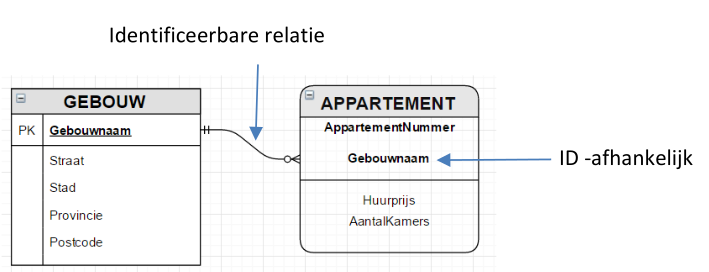
\includegraphics[width=0.7\textwidth]{Screenshot_20200325_135140.png}
    \caption{Identificeerbare relatie. Voorstelling: met een volle lijn.}
\end{figure}

\subsubsection{Niet-identificeerbare relaties}
Kan zelfstandig geïdentificeerd worden zonder een aanwezige parent. De PK van de
afhankelijke entiteit kan zo een eigen serienummering zijn, zonder enig verband met
een andere entiteit. Zo heeft een boek een aantal lezers als niet-identificeerbare relatie,
want de lezer heeft nergens een eenduidige referentie naar 1 boek. 

\underline{Voorbeeld:} Een VIN (Vehicle Identification Number) bevat in volgend model geen
verwijzing naar het model. De 'Wagen' entiteit verwijst nergens in de benaming van zijn
attributen naar de 'Model' entiteit. Vanuit de wagen entiteit kan het model van de fabrikant
niet worden geïdentificeerd.

\begin{figure}[H]
    \centering
    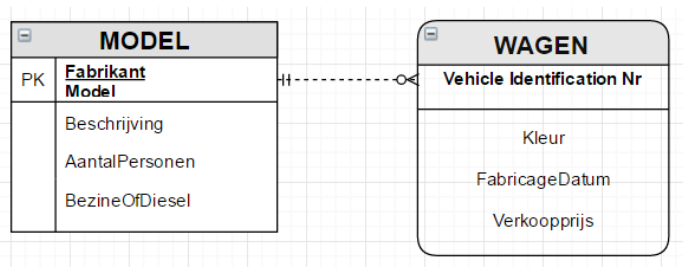
\includegraphics[width=0.6\textwidth]{Screenshot_20200325_180636.png}
    \caption{Niet-dentificeerbare relatie. Voorstelling: met een stippelijn.}
\end{figure}

\subsection{Grafische voorstelling van een ER-model}
Het ER-model wordt voorgesteld (getekend), deze voorstelling heet een \bold{Entiteit Relatie Diagram (ERD)}
Er bestaan vele vormen van deze grafische voorstelling. Verschillende softwarepakketen zijn beschikbaar:

\begin{itemize}
    \item IDEF1X = Integrated DEFinition Extended. Amerikaans, wereldwijd erkend, complex
    \item UML = Unified Modeling Language = voor object georiënteerde programmeertalen. 
    Er worden meerdere types diagrammen gedefinieerd (structuurdiagrammen, behaviour diagrammen)
\end{itemize}

\subsubsection{Het kraaienpootmodel}

De kraaienpoot toont waar meerdere gerelateerde entiteiten mogelijk zijn. De 0 staat voor optioneel
(minimaal 0 gerelateerde entiteiten), de | staat voor required (minimaal 1 gerelateerde entiteit)

\begin{itemize}
    \item De 0 of | die \bold{verst van de entiteit} staat (meer in de midden), toont de \bold{minimale kardinaliteit}
    \item De 0 of | die \bold{dichtst bij de entiteit} staat, toont de \bold{maximale kardinaliteit}
\end{itemize}


\begin{figure}[H]
    \centering
    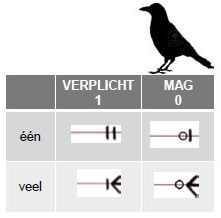
\includegraphics[width=0.3\textwidth]{kraaienpootmodel.png}
    \caption{Kraaienpootmodel}
\end{figure}

\bold{Voorbeeld}: 1 customer kan meerdere contracten hebben. Een customer hoeft geen contract te
hebben, maar een contract heeft minimaal 1 customer. Dit kan op verschillende manieren worden voorgesteld. 

\begin{figure}[H]
    \centering
    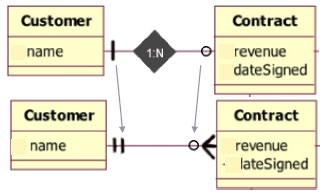
\includegraphics[width=0.5\textwidth]{kraaienpootmodel-voorbeeld.png}
    \caption{Voorbeeld kraaienpootmodel}
\end{figure}

\bold{Noot:} Blijf bij het aanmaken van het model op de gebruikte taal en blijf consequent:
duidelijke namen, kies voor 1 bepaalde opbouw, \dots. Bv: alles in het engels, een ID met hoofdletters,
camelCasing of snake\_casing, \dots

\subsection{Tekenen van het ERD model in de praktijk}

\begin{itemize}
    \item Vaak op papier
    \item In bijzijn van de klant
    \item Kan ook via tekentools (draw.io, Visio van MS Office, MySQL Workbench)
\end{itemize}

\subsection{Model voorbeeld 1: Gerechten en hun categorie bij de recipesdb}

\underline{Gegeven:} Een FoodCategory kan meerdere Recipes bevatten. Een FoodCategory hoeft geen Recipe te bevatten.

\subsubsection{Het model}

\begin{figure}[H]
    \centering
    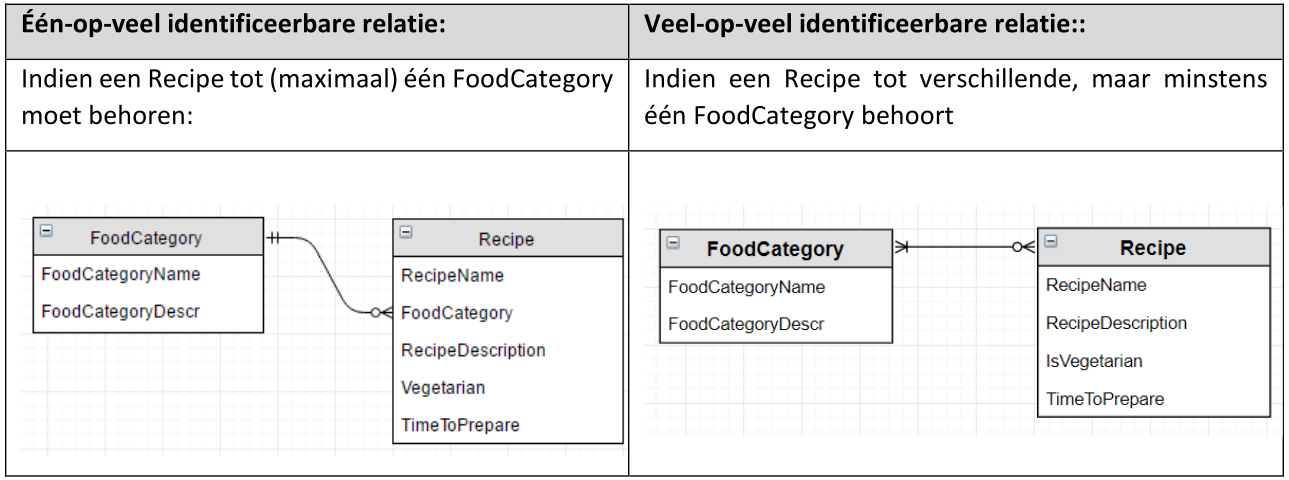
\includegraphics[width=0.9\textwidth]{Screenshot_20200401_134247.png}
    \caption{De databasemodellen zien er minstens zo uit}
\end{figure}

Gedurende het gesprek met een klant kan dit basismodel evolueren naar het ontwerp toe.
Of je kiest ervoor om voor jezelf een tweede model te tekenen, waar meer ontwerpgegevens
in voorkomen: datatypes, defaultwaarden, keys \dots

\subsubsection{Het ontwerp}
Finaal zal dit model toch een database ontwerp worden met een volledig uitgetekend en gedetailleerd ERD.

\underline{Voorbeeld: } in bovenstaand model krijgen in het ontwerp beide entiteiten 
(FoodCategory en Recipe) een identity kolom (ook surrogaatsleutel genoemd) als determinant:

\begin{figure}[H]
    \centering
    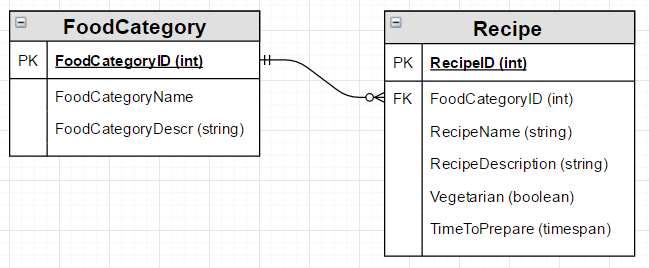
\includegraphics[width=0.7\textwidth]{databaseontwerp.png}
    \caption{1-op-veel}
\end{figure}

\begin{figure}[H]
    \centering
    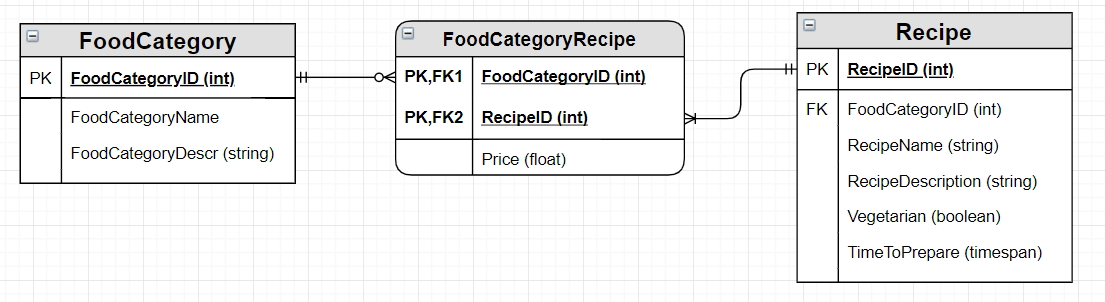
\includegraphics[width=0.7\textwidth]{veel-op-veel.png}
    \caption{veel-op-veel (met tussentabel)}
\end{figure}


\subsection{Model voorbeeld 2: Distributie van producten}

\underline{Gegeven: } een spreadsheet met productinformatie en dealerinformatie:

\begin{itemize}
    \item De product informatie bevat: aanbevolen eindgebruikerprijzen , productnaam , ID, voorraad
    \item De dealer informatie bestaat uit: dealernaam, zijn contactgegevens (plaats, land) en het aantal bestelde producten samen met hun verkooprijs.
\end{itemize}

\begin{figure}[H]
    \centering
    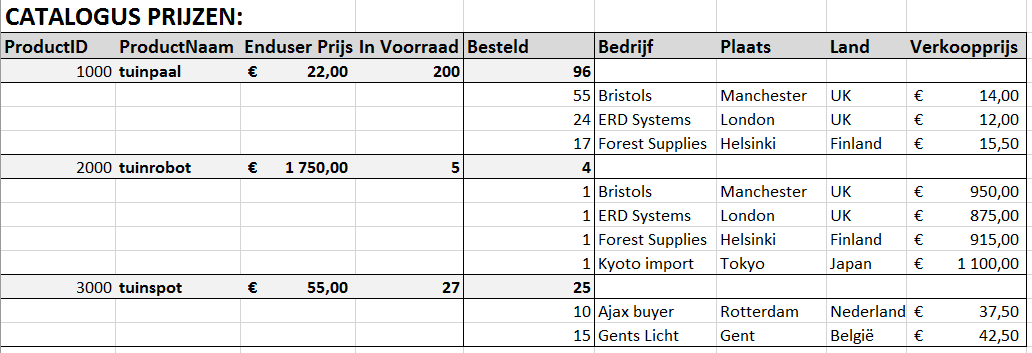
\includegraphics[width=0.7\textwidth]{model2.png}
    \caption{De spreadsheet}
\end{figure}

\subsubsection{Het model}

\begin{figure}[H]
    \centering
    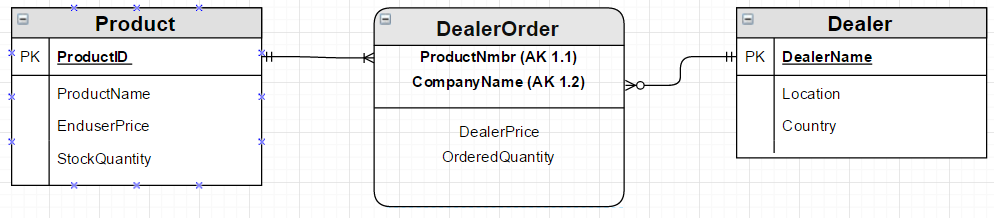
\includegraphics[width=0.7\textwidth]{model2-model.png}
    \caption{Het resulterende model (1 van de mogelijkheden)}
\end{figure}


\section{Een ACID database ontwerp}

\subsection{Definitie ACID}

\bold{ACID} staat voor Atomic - Consistent - Isolated - Durable.

\begin{itemize}
    \item \underline{\bold{Atomic}}: Alles of niets: als een deel van de transactie faalt, faalt de volledige transactie
    \item \underline{\bold{Consistent}}: Wat de transactie ook is, de database behoudt zijn gevalideerde structuur en status.
    \item \underline{\bold{Isolated}}: elke transactie gebeurt los van elkaar en interfereert niet met elkaar. De ene transactie weet niet hoe de andere transactie verloopt.
    \item \underline{\bold{Durable}}: Eenmaal een transactie succesvol voltooid is, resulteert dit een wijziging op de database die blijvend is (=data overleeft een crash, bestaat niet enkel vluchtig in het geheugen)
\end{itemize}

\subsection{Stappen bij het ontwerpen van een ACID database}
\begin{itemize}
    \item Tabellen maken op de database server voor elke entiteit
    \item Sleutels (PK, FK) worden aangemaakt
    \item Extra tabellen worden toegevoegd om veel-op-veel relaties te ondersteunen en zo tot een genormaliseerde (ACID) database te komen
    \item Attributen van de entiteit worden eigenschappen (kolommen) in de tabel.
    \item Vastleggen van specificaties zoals: al dan niet nullable, datatype, constraints, defaultwaarden
    \item Leggen van de relaties tussen tabellen: 1:1, 1:N, N:M. Veel aandacht naar \bold{referentiële integriteit}. 
    \item Veel-op-veel relaties resulteren altijd in een tussentabel (!). De tussentabel heeft vaak de primaire sleutels van beide refererende tabellen opgenomen. 
\end{itemize}

\subsubsection{Referentiële integriteit}
\begin{itemize}
    \item PK en FK moeten van hetzelfde datatype zijn
    \item FK bestaat altijd maar kan/mag een waarde null hebben (=controleren op null)
    \item Je kan een PK niet verwijderen als er nog gerelateerde FK records zijn 
\end{itemize}

Hoe een PK verwijderd wordt samen met zijn afhankelijkheden kan je kiezen:
\begin{itemize}
    \item Cascade
    \item Set NULL
    \item Restrict
    \item Je kan een FK pas toevoegen als er een gerelateerde PK bestaat. Je moet dus eerst de PK aanmaken
\end{itemize}

\section{Normalisatie}
\subsection{Wat?}
\begin{itemize}
    \item Na het wijzigen van data in het relationele model kunnen sommige tabellen fouten bevatten (verwijderanomalieën, invoeganomalieën)
    \item Oplossing: normaliseren
    \item Ontstaan in 1973 tijdens de groei van relationele databases
    \item Dr. Edgar Codd definieerde de normaalvorm 
\end{itemize}

\subsection{Voordelen}

\begin{itemize}
    \item Verwijdert wijzigingsanomalieën
    \item Voorkomt dubbele gegevens
    \item Voorkomt integriteitsproblemen
    \item Spaart opslagruimte uit (gezien er geen herhalingen zijn).
\end{itemize}

\subsection{Nadelen}

\begin{itemize}
    \item Ingewikkelder SQL om gegevens uit verschillende tabellen te verwijderen.
    \item Een extra key kan nodig zijn, om bijna gelijke waarden te kunnen wegschrijven. Aanpassen van een database is niet eenvoudig met al die tabellen en kan resulteren in minder goede performantie.
    \item Relaties worden onderworpen aan constraints (beperkingen, regels)-> vraagt DBkennis
    \item Meer tabellen betekent extra zoekwerk voor het DBMS (database management system), wat de snelheid kan doen dalen.
\end{itemize}


\subsection{Normaalvormen}
Een normaalvorm kan je zien als een kwaliteitsindicatie van een database. Er zijn 5 basisnormaalvormen:

\begin{itemize}
    \item 1NF ("first normalform")
    \item 2NF
    \item 3NF
    \item BCNF of 3.5NF
    \item 4NF
\end{itemize}

4NF voldoet ook aan BCNF, wat ook voldoet aan 3NF, wat ook voldoet aan 2NF, \dots

\subsection{Voorbeeldoefening}

In volgende tabel zijn veel herhalingen aanwezig, die we \bold{redundant} of \bold{overtollig} noemen.
De PK is (EntryDate, Category, Name). 

\begin{figure}[H]
    \centering
    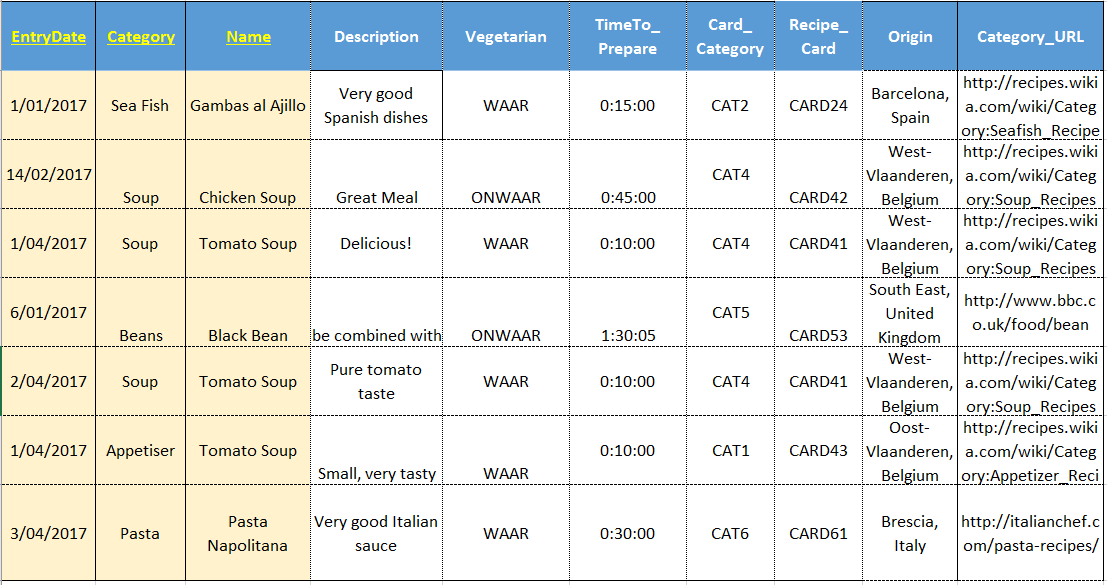
\includegraphics[width=\textwidth]{0NF.png}
    \caption{Niet-genormaliseerde tabel (0NF)}
\end{figure}


\subsubsection{1NF}
1NF concentreert zich op samengestelde attributen en herhalingen van attributen
\begin{itemize}
    \item Geen samenstelling in attributen (er worden atomaire attributen verwacht)
    \item Geen herhalingen van gelijk(w)aardige attributen of attribuuttypes
\end{itemize}

In de oefening kunnen we 2 dingen veranderen om de normaalvorm te verhogen:

\begin{itemize}
    \item Card\_Category komt overeen met Category. Een ervan mag verwijderd worden
    \item Het 'Origin' attribuut is samengesteld. We kunnen het splitsen onder 2 afzonderlijke attributen: 'Province' en 'Country'
\end{itemize}

\begin{figure}[H]
    \centering
    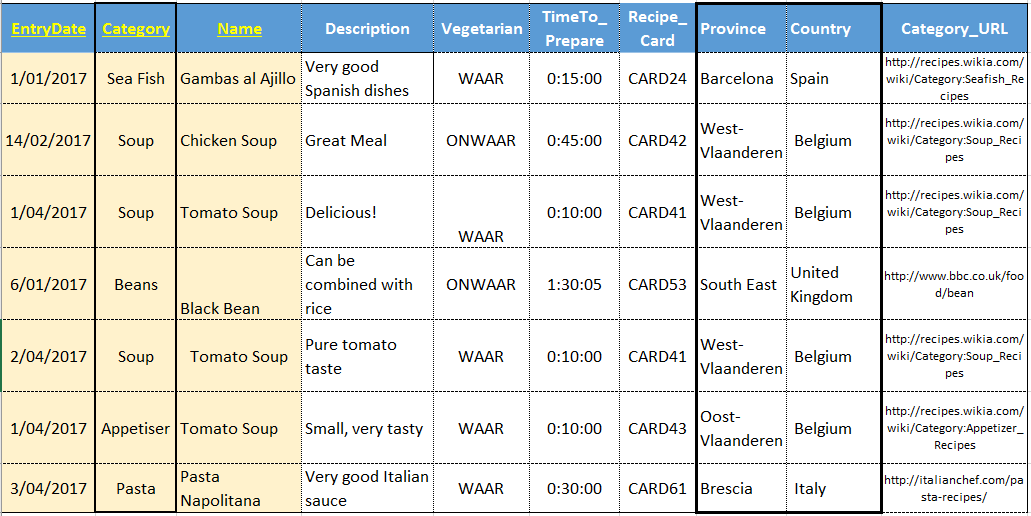
\includegraphics[width=\textwidth]{1NF.png}
    \caption{Genormaliseerd tot 1NF}
\end{figure}

\subsubsection{2NF}
2NF concentreert zich op de anomalieën die ontstaan door afhankelijkheden van de (samengestelde) PK.
\begin{itemize}
    \item De tabel staat in 1NF
    \item Elk attribuut die niet in de primary key zit is afhankelijk van de volledige (!) samengestelde primary key 
\end{itemize}

In de oefening:

\begin{itemize}
    \item Category\_URL is enkel afhankelijk van het PK-deel Category en niet van de volledige (!) samengestelde PK. 
    Category en Category\_URL moeten we daarom overbrengen naar een nieuwe tabel
\end{itemize}

\begin{figure}[H]
    \centering
    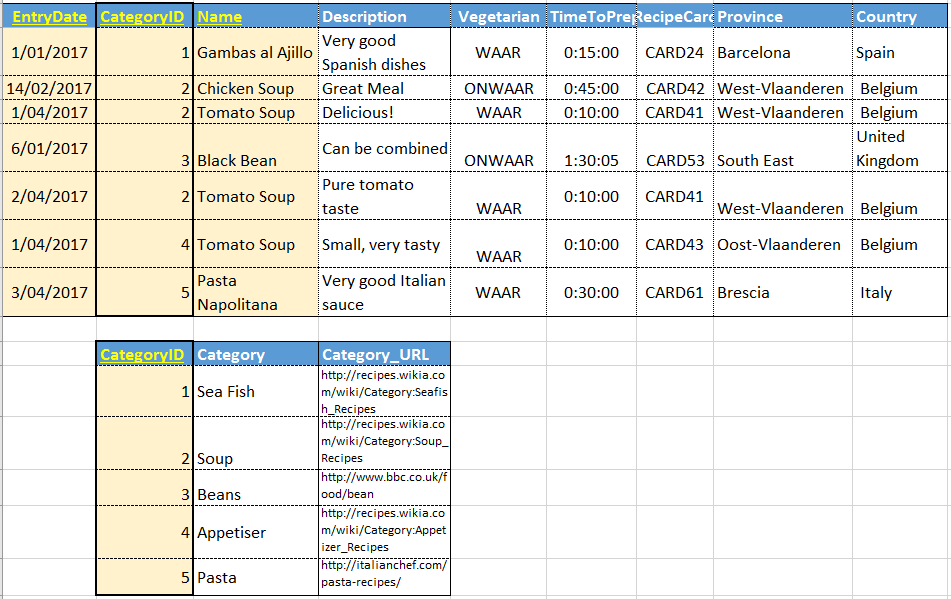
\includegraphics[width=0.8\textwidth]{2NF.png}
    \caption{Genormaliseerd tot 2NF}
\end{figure}

\subsubsection{3NF}
3NF concentreert zich op anomalieën die ontstaan door afhankelijkheden bij de niet-primaire key attributen
\begin{itemize}
    \item De tabel staat in 2NF
    \item Geen enkele niet-primaire kolom is functioneel afhankelijk van een andere niet-primaire sleutel kolom. 
    \item De niet-primaire attributen hangen alleen af van de volledig samengestelde key.
    \item Transitiviteit kan niet in 3NF! (=kolommen die niet direct afhankelijk zijn van de PK maar bijvoorbeeld wel van een andere attribuut)
\end{itemize}

In deze oefening: Provincie en land zijn transitief (onderling afhankelijk) $\Rightarrow$ worden afgesplitst

\begin{figure}[H]
    \centering
    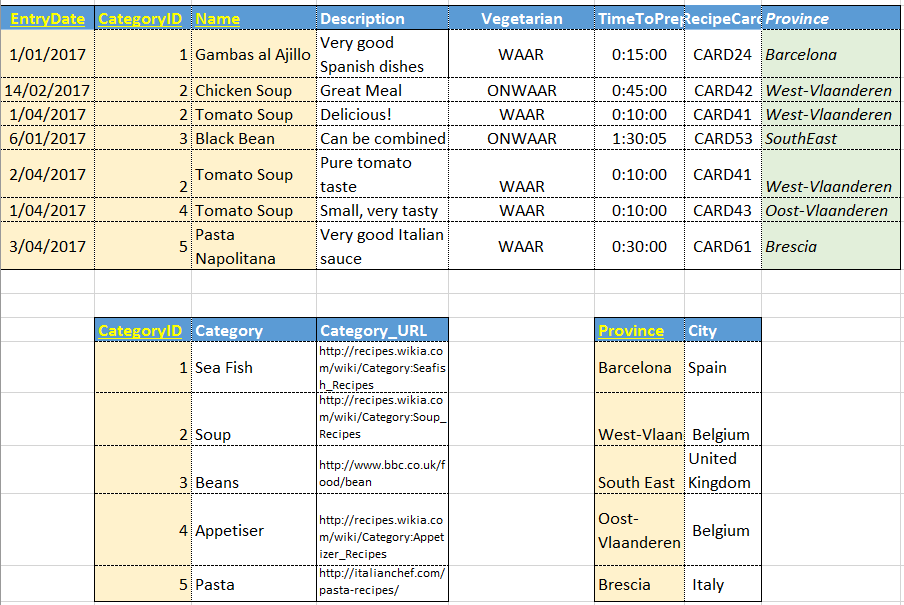
\includegraphics[width=0.8\textwidth]{3NF.png}
    \caption{Genormaliseerd tot 3NF}
\end{figure}

\subsubsection{BCNF (3.5NF)}
BCNF concentreert zich op de determinanten die geen kandidaatsleutel zijn.
\begin{itemize}
    \item De tabel staat in 3NF
    \item Elke mogelijke determinant (=alternatieve key) is een kandidaatsleutel
    \item Als er maar 1 kandidaatsleutel is, dan staat een 3NF relatie automatisch in BCNF
    \item Splits elke determinant af die geen kandidaatsleutel is, maar toch functioneel afhankelijk is, in een afzonderlijke tabel.
\end{itemize}

In deze oefening:

\begin{itemize}
    \item RecipeCard kan als een determinant CardID beschouwd worden van een andere tabel, 
    en CardID is op zich geen kandidaatsleutel (2x dezelfde waarde CARD41). We splitsen dus CardID af
    \item Als afwerking kan nu ook een RecipeID als PK worden toegevoegd.
\end{itemize}

\begin{figure}[H]
    \centering
    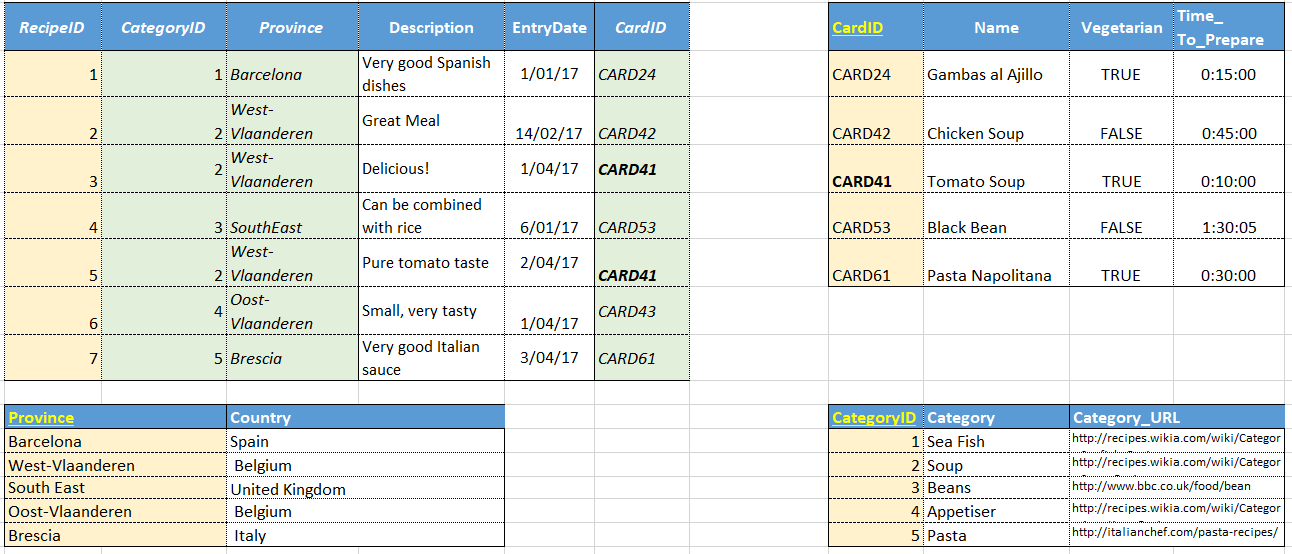
\includegraphics[width=\textwidth]{BCNF.png}
    \caption{Genormaliseerd tot BCNF}
\end{figure}

\subsubsection{4NF en 5NF}
4NF en 5NF concentreren zich op meerwaardige afhankelijkheden. Het verschil met BCNF 
wordt alleen duidelijk als er meerwaardige afhankelijkheden zijn. 

Een \bold{meerwaardige
afhankelijkheid} betekent dat bij het toevoegen van een item, ook andere gegevens
in andere kolommen van dezelfde tabel moeten worden overgenomen ook al zijn ze 
functioneel onafhankelijk van de wijziging.

\begin{figure}[H]
    \centering
    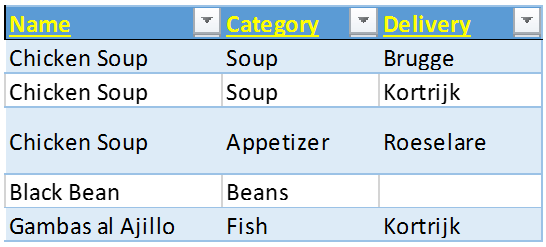
\includegraphics[width=0.4\textwidth]{4NFvoorbeeld.png}
    \caption{BCNF-tabel}
\end{figure}

Als je in deze tabel een nieuwe delivery toevoegt, (vb Gent) dan moet ook Name
en Category overgekopieerd worden, ook al heeft Delivery niets met Category te maken.

Oplossing: een tabel Name/Category en een tabel Name/Delivery maken. Dan staat de tabel in 4NF

5NF zoekt in de meerwaardige afhankelijkheden naar een logische samenhang van 
de kandidaatsleutels door domeinen ervoor te beschouwen of randvoorwaarden aan te
brengen. 5NF zien we niet in deze module.

\subsection{Normaalvormen overzicht}

\begin{figure}[H]
    \centering
    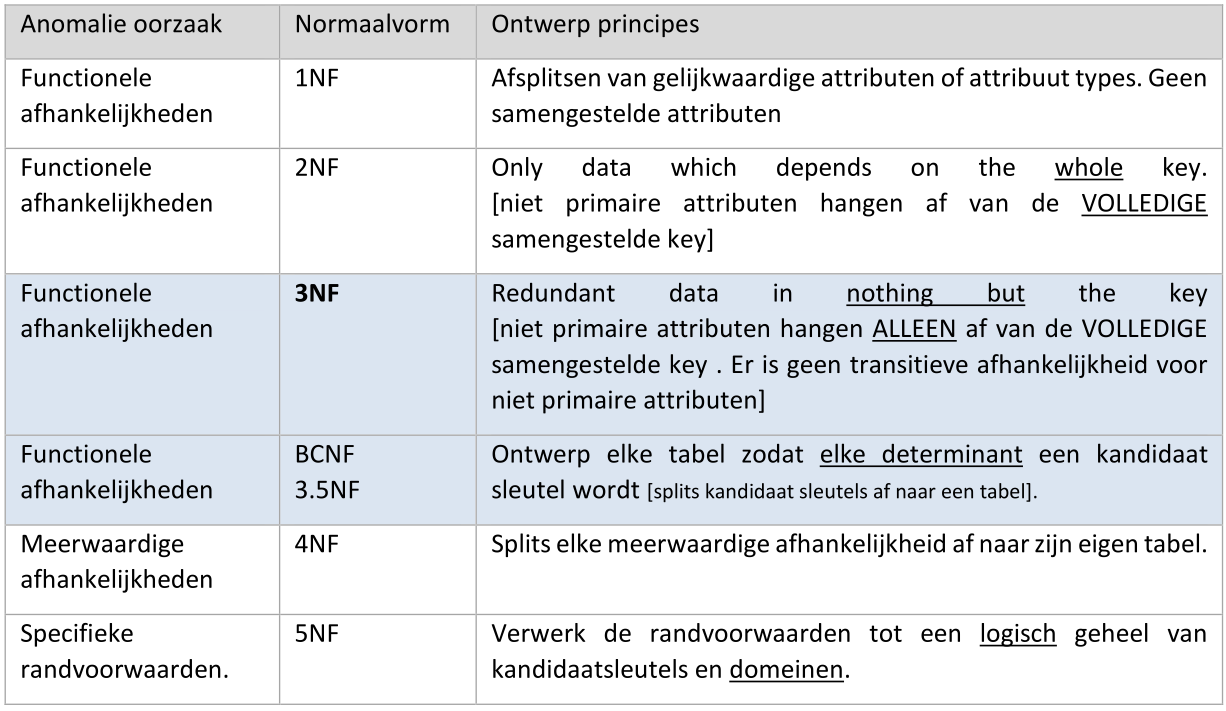
\includegraphics[width=\textwidth]{Screenshot_20200325_175126.png}
    \caption{Overzicht}
\end{figure}

We gebruiken altijd 3NF en streven naar BCNF. Om BCNF te realiseren gebruik je deze regel:

\begin{itemize}
    \item Ontwerp de tabellen zodat elke determinant een kandidaatsleutel is. 
    \item Splits daarna zoveel mogelijk afhankelijkheden af in verschillende tabellen.
\end{itemize}

Het toepassen van normalisatie resulteert in een \bold{ACID} database model/ontwerp.

\section{Data Definition Language (DDL)}
We hebben een database server geïnstalleerd (MySQL en/of MSSQL) en 
we hebben een genormaliseerd ontwerp. Nu kunnen we met T-SQL en met visuele editors de database realiseren 

\subsection{Het ontwerp realiseren met de taal T-SQL}
Referenties: 

\begin{itemize}
    \item Handige, korte referentie: \url{http://www.w3schools.com/sql/sql_quickref.asp}
    \item Volwaardige MSSQL referentie: \url{https://msdn.microsoft.com/en-us/library/bb510741.aspx}
    \item Volwaardige MySQL referentie: \url{http://dev.mysql.com/doc/refman/8.0/en/sql-syntax.html}
\end{itemize}

Let op het onderscheid tussen DDL en DML:

\subsubsection{DDL (= Data Definition Language)}
DDL wordt gebruikt om op basis van een database structuur (ERD, EnhancedERD, UML) de werkelijke
database (genaamd 'schema' in MySQL) aan te maken. DDL laat ook toe om een bestaande
structuur aan te passen, te verwijderen, inhoud te verwijderen, \dots

\begin{figure}[H]
    \centering
    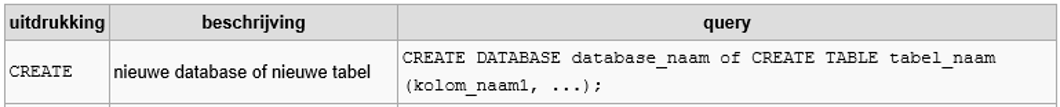
\includegraphics[width=\textwidth]{ddl-acties.png}
    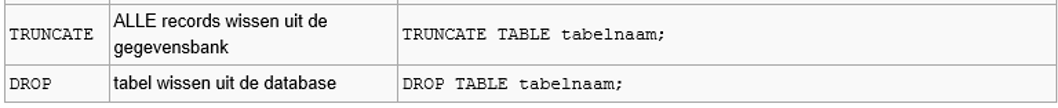
\includegraphics[width=\textwidth]{ddl-acties2.png}
    \caption{DDL acties}
\end{figure}

\subsubsection{DML (= Data Manipulation Language)}
Met DML kan de data zelf in de database behandeld worden (CRUD-acties).

Zowel DDL als DML kunnen op verschillende manieren aangemaakt of uitgevoerd worden:

\begin{enumerate}
    \item Zelf T-SQL in een query venster schrijven
    \item T-SQL door een tool (het DBMS) te laten genereren en uit te voeren.
    \item Door een applicatie (in Python, Java, C\#, \dots) die via libraries T-SQL naar een server kan sturen
\end{enumerate}

\begin{figure}[H]
    \centering
    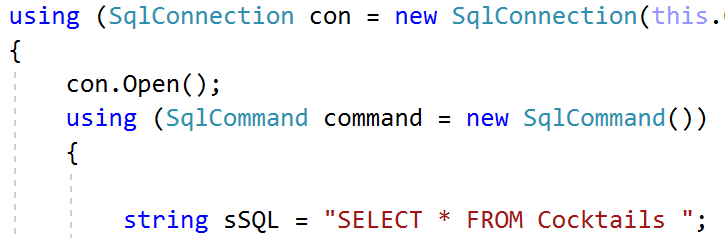
\includegraphics[width=0.6\textwidth]{t-sql-csharp.png}
    \caption{Voorbeeld in C\#}
\end{figure}

\subsection{Het ontwerp realiseren met een visuele editor}
We tekenden ons ontwerp in een losstaand programma; maar de “MySQL Workbench” beschikt ook over een
visuele editor.

\subsubsection{Forward Engineering}

\begin{itemize}
    \item Je tekent het genormaliseerd model (ERD of Schema) met zijn relaties -> je krijgt een EERD (Enhanced ERD).
    \item Je genereert de database vanuit het getekend model
    \item Na wijzigingen aan getekend model of wijzigingen aan de database mag je niet vergeten beide te synchroniseren.
\end{itemize}

\subsubsection{Reserverse engineering}
\begin{itemize}
    \item Je maakt een genormaliseerde relationele database aan met T-SQL via DDL.
    \item Of: je beschikt over een database in de vorm van een script of in de vorm van een backupfile en restoret deze database op de server.
    \item Je genereert het getekend model (ERD of Schema) vanuit de bestaande relationele database.
\end{itemize}

\begin{figure}[H]
    \centering
    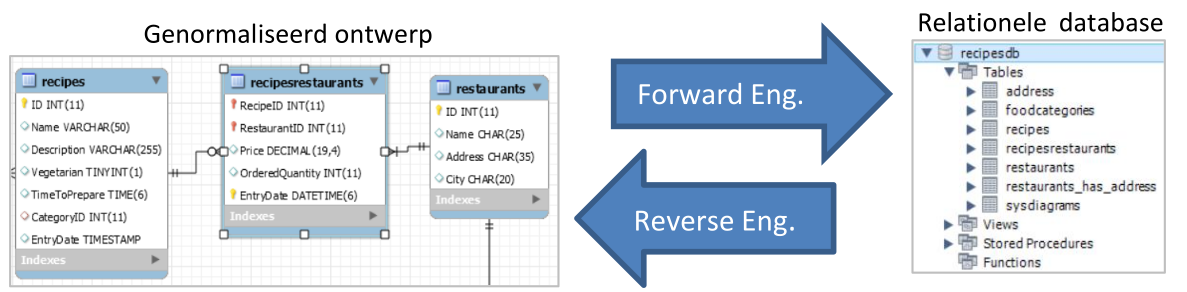
\includegraphics[width=0.9\textwidth]{forward-backward-engineering.png}
    \caption{Forward \& Backward Engineering}
\end{figure}

\subsection{DDL instructies}
\subsubsection{CREATE TABLE in MySQL}
\begin{figure}[H]
    \centering
    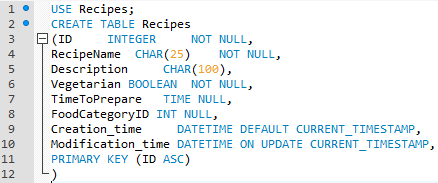
\includegraphics[width=0.6\textwidth]{create-table.png}
    \caption{CREATE TABLE in MySQL}
\end{figure}

\subsubsection{DDL met MySQL}
\begin{figure}[H]
    \centering
    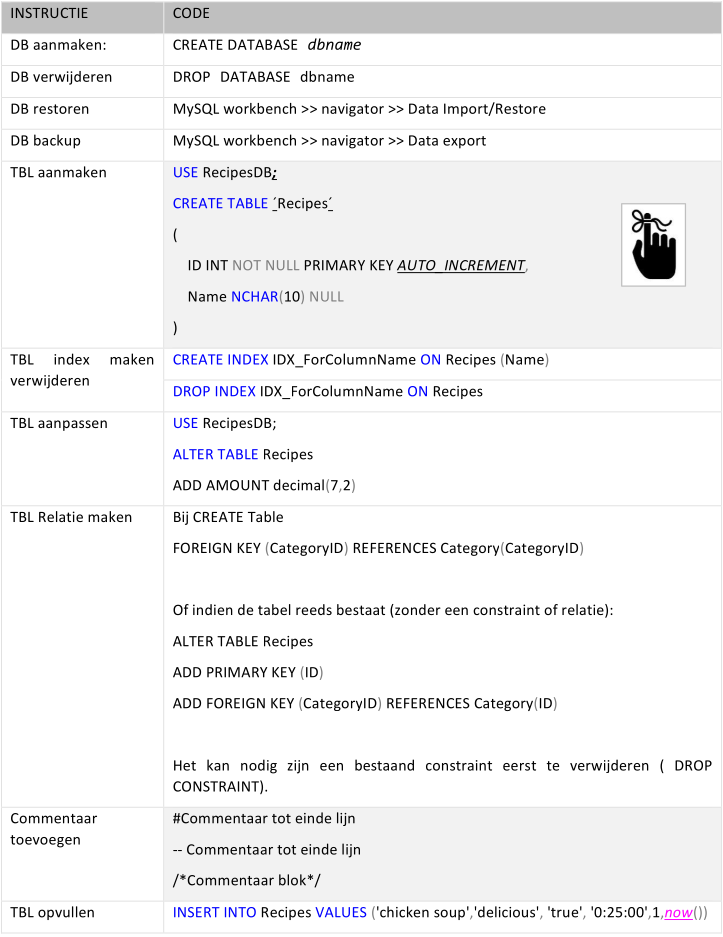
\includegraphics[width=0.95\textwidth]{overzicht-ddl.png}
    \caption{Overzicht DDL}
\end{figure}

Het opvullen van de tabellen (INSERT INTO) is eigenlijk DML, maar wordt toch heel vaak gebruikt in DDL.

Merk op: in MSSQL wordt een boolean voorgesteld als een string 'true' of 'false', terwijl
in MySQL een boolean wordt voorgesteld als TRUE of FALSE (zonder quotes). 

\subsubsection{Datatypes}
\begin{figure}[H]
    \centering
    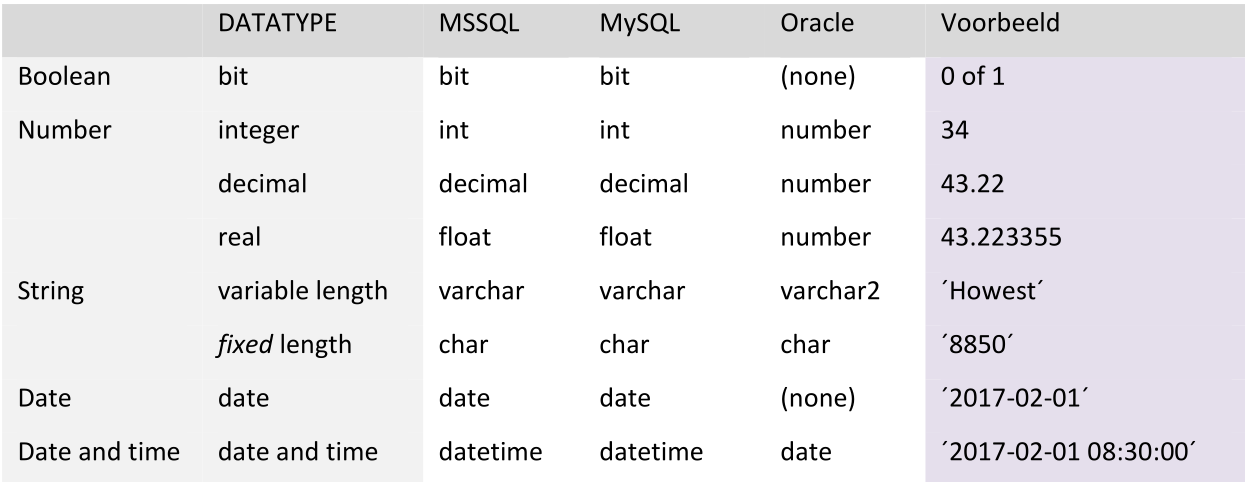
\includegraphics[width=0.9\textwidth]{overzicht-datatypes.png}
    \caption{Overzicht datatypes}
\end{figure}

\begin{itemize}
    \item CHAR is typisch voor MSSQL en MySQL en verwijst naar een vaste lengte. De spaties blijven bewaard.
    \item VARCHAR is voor een variabele lengte van maximum 8bit (UTF8 of 255 karakters)
    \item NVARCHAR(size) enkel bij MSSQL is dan weer voor volwaardige Unicode. Het karakter “N” (zoals bij NVARCHAR) verwijst in SQL vaak naar Unicode als encodeersysteem.
\end{itemize}

Een volledig overzicht van de datatypes is te vinden in de referenties: \url{https://dev.mysql.com/doc/refman/8.0/en/data-types.html}

\subsubsection{Indexen}
\begin{itemize}
    \item Versnelt zoekacties
    \item De index is niet noodzakelijk de PK! Meestal worden indexen geplaatst op zowel de PK als de FKs
    \item Meestal toegekend via de contextmenus van de visuele editor (MySQL workbench)
    \item Naam van de index heeft als suffix '\_idx'
\end{itemize}
\bold{Verschillende index types:}
\begin{itemize}
    \item Clustered of niet clustered
    \begin{itemize}
        \item Clustered index (meest gebruikt) = kolomnamen ingesloten in de indexdefinitie zorgen voor een sortering van de rijen
        \item Non-clustered = een afzonderlijke structuur met pointers zorgt voor de sortering 
    \end{itemize}
    \item dalend (descending) of stijgend(ascending)
    \item UNIEK of niet uniek
    \begin{itemize}
        \item uniek: data van de volledige index mag slechts 1x voorkomen
    \end{itemize}
    \item FULLTEXT index
    \begin{itemize}
        \item laat full-text queries toe = er wordt gezocht naar woorden en zinnen ipv enkele karakters
    \end{itemize}
    \item SPATIAL index
    \begin{itemize}
        \item wordt gebruikt bij queries op geometrische en geografische data zoals coördinaten.
    \end{itemize}
\end{itemize}

\bold{Voorbeeld index aanmaken via wijziging (ALTER)}

\begin{lstlisting}[language=SQL]
ALTER TABLE `dbname`.`persons`
    ADD COLUMN `FirstName` VARCHAR(45) NOT NULL AFTER `ID`,
    ADD COLUMN `LastName` VARCHAR(45) NOT NULL AFTER `FirstName`,
    ADD UNIQUE INDEX `Name` (`FirstName` ASC, `LastName` ASC);
\end{lstlisting}

\subsubsection{Constraints}
Door het aanmaken van relaties worden “foreign key constraints” actief. 
Dit zorgt ervoor dat de database referentieel integer blijft en is dus een must bij relationele databasen.

Na het leggen van de relaties kan je geen record verwijderen als er nog relationele records voor bestaan. 
Je moet eerst de relationele records verwijderen. Dit gedrag kan je veranderen of instellen via 4 parameters:

\begin{itemize}
    \item RESTRICT in MySQL of NO ACTION in MSSQL
    \begin{itemize}
        \item Je verwacht dat de referentiële integriteit bewaard wordt, zonder dat automatische acties uitgevoerd worden op child records
    \end{itemize}
    \item CASCADE
    \begin{itemize}
        \item Alle child records worden aangepast of verwijderd wanneer de parent aangepast of verwijderd wordt
    \end{itemize}
    \item SET NULL
    \begin{itemize}
        \item De FK kolom of kolommen bij de child records worden op NULL geset.
    \end{itemize}
    \item SET DEFAULT
    \begin{itemize}
        \item De FK-kolom of kolommen bij de child records worden ingesteld op de default waarde.
    \end{itemize}
\end{itemize}


\bold{Voorbeeld in T-SQL:} een wijziging waarbij met een delete of update alle child records aangepast worden.(=gevaarlijk en niet aangeraden)

\begin{lstlisting}[language=SQL]
ALTER TABLE dbo.Table1
    ADD CONSTRAINT FK_Table1_Table2
    FOREIGN KEY(Table2ID) REFERENCES dbo.Table2(ID)
        ON DELETE CASCADE
        ON UPDATE CASCADE
\end{lstlisting}

\bold{\underline{Opmerking:}} 
Pas sedert MySQL 5.5 worden foreign-key constraints ondersteund door de actuele InnoDB engine van MySQL. 


\subsection{Reverse engineering met MySQL Workbench tools}
De meeste DDL-taken kunnen uitgevoerd worden in MySQL workbench zonder dat je zelf T-SQL schrijft, via contextmenu's (rechtermuisknop).
Dit is dan ook de meest gebruikte manier om een database via reverse engineering aan te maken.

Zaken die sowieso bijna altijd via de contextmenu's worden gedaan:

\begin{itemize}
    \item archiveren
    \item restoren
    \item instellen van indexen
    \item instellen van constraints op relaties
\end{itemize}


\subsubsection{Overzicht reverse engineering}
\begin{figure}[H]
    \centering
    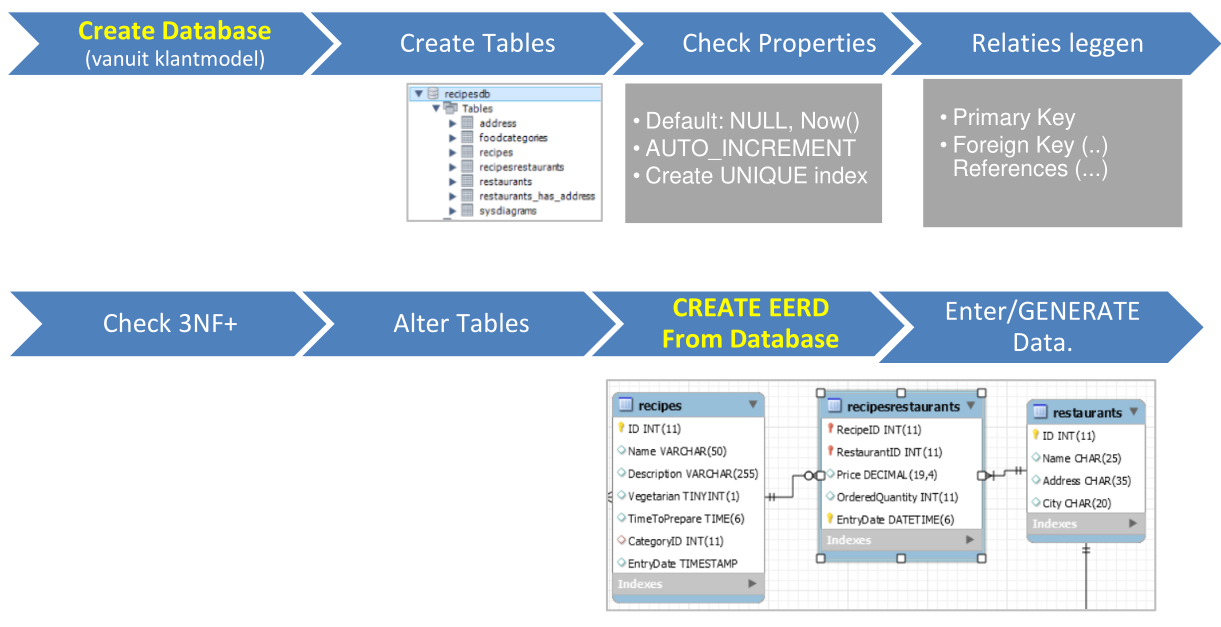
\includegraphics[width=0.9\textwidth]{overzicht-reverse-engineering.png}
    \caption{Overzicht reverse engineering}
\end{figure}

\subsubsection{Stappenplan}
Via het recipesdb voorbeeld:

\begin{figure}[H]
    \centering
    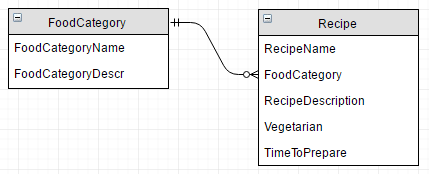
\includegraphics[width=0.6\textwidth]{recipesdb.png}
    \caption{Genormaliseerd model}
\end{figure}

\begin{enumerate}
    \item Lokale MySQL server instantie starten
    \item Open Workbench en klik de connectie om de lokale instantie van de server te openen
    \item Maak een nieuw schema aan 'recipesdb': rechtermuisklik in het Schema venster aan de linkerkant en druk op 'Create Schema...'. Refresh het Schemas venster
    \item Open recipesdb en maak via een rechtermuisklik op zijn Tables de tabel 'foodcategories' aan. We gebruiken als engine 'InnoDB'.

    \begin{figure}[H]
        \centering
        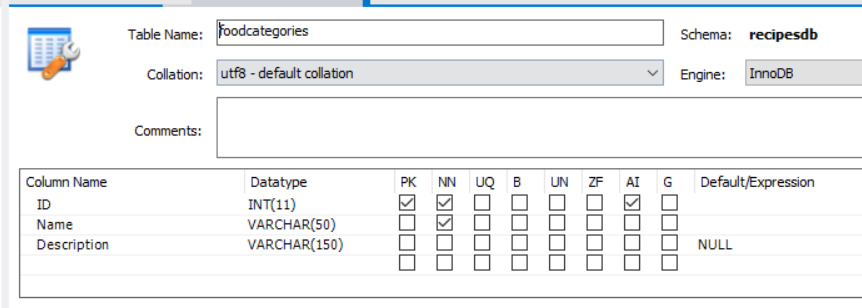
\includegraphics[width=0.6\textwidth]{stappenplan-1.png}
        \caption{Aanmaak tabel 'foodcategories'. Druk op Apply.}
    \end{figure}

    \item Maak nu ook de tabel recipes aan volgens het model.
    \item Maak de relaties aan om de database referentieel integer te houden
    \begin{itemize}
        \item Rechtermuisklik op een tabel $\Rightarrow$ alter table \dots $\Rightarrow$ nu zit je in 'design mode'
        \item Klik onderaan op de tab 'Foreign Keys'
        \item Maak een nieuwe foreign key aan
    \end{itemize}

    \begin{figure}[H]
        \centering
        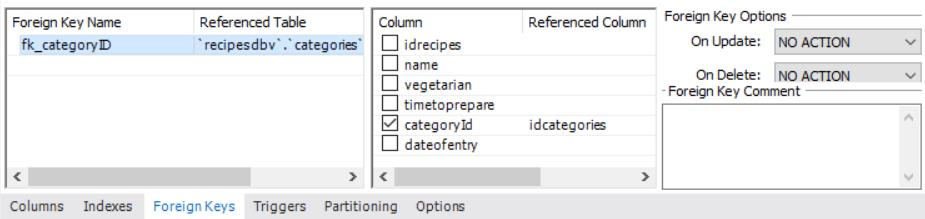
\includegraphics[width=0.7\textwidth]{stappenplan-2.png}
        \caption{Aanmaak relatie}
    \end{figure}

    \begin{figure}[H]
        \centering
        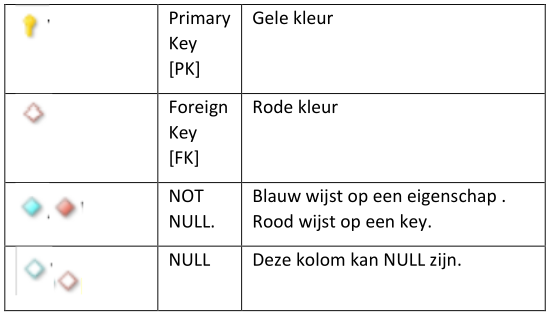
\includegraphics[width=0.4\textwidth]{symbolen.png}
        \caption{De symbolen}
    \end{figure}

    \item Indexen toevoegen voor unieke data in kolommen en voor snellere zoekacties.
    \begin{itemize}
        \item Je kan de sorterin instellen: stijgend/dalend
        \item Je kan meerdere kolommen kiezen voor eenzelfde index
    \end{itemize}
    \begin{figure}[H]
        \centering
        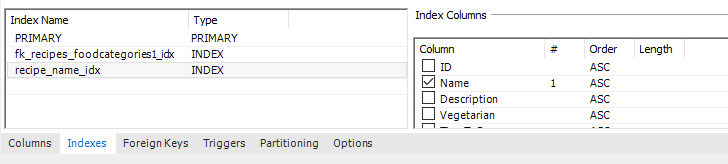
\includegraphics[width=0.7\textwidth]{stappenplan-3.png}
        \caption{Aanmaak indexen}
    \end{figure}

    \item Voer manueel wat testdata op in beide tabellen (Recipe en FoodCategory)
    \item Het model (EERD) tekenen/genereren vanuit de gemaakte database (=reverse engineering)

    \begin{figure}[H]
        \centering
        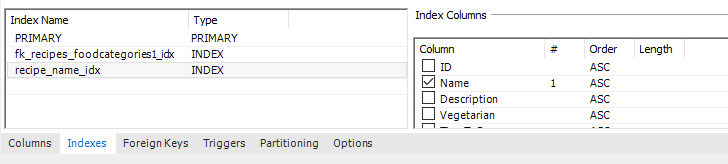
\includegraphics[width=0.7\textwidth]{stappenplan-3.png}
        \caption{Home page MySQL workbench $\Rightarrow$ Create EER model from Database}
    \end{figure}

    \item Aangemaakt model (EERD) controleren en aanpassen waar nodig.
    \item Database (Schema) synchroniseren met het gewijzigd model
    \begin{itemize}
        \item Model en database zijn niet automatisch gelinkt met elkaar.
        \item Je moet zelf een synchronisatie doen via de menu item:
        \item Workbench >> Database >> Synchronize Model (CTRL + SHIFT + Z).
    \end{itemize}
    \item Model (EERD) bewaren voor later gebruik: Workbench >> File >> Save of WorkbenchFile >> Save As >> *.mwb
\end{enumerate}

\subsubsection{Testdata genereren met een tool}
Manier om testdata aan te maken om te gebruiken in een database: \url{http://www.generatedata.com/}

\subsection{Forward engineering met MySQL Workbench tools}
Forward engineering verwacht dat we eerst het (genormaliseerde) model tekenen om daarna de database eruit te genereren.

\begin{figure}[H]
    \centering
    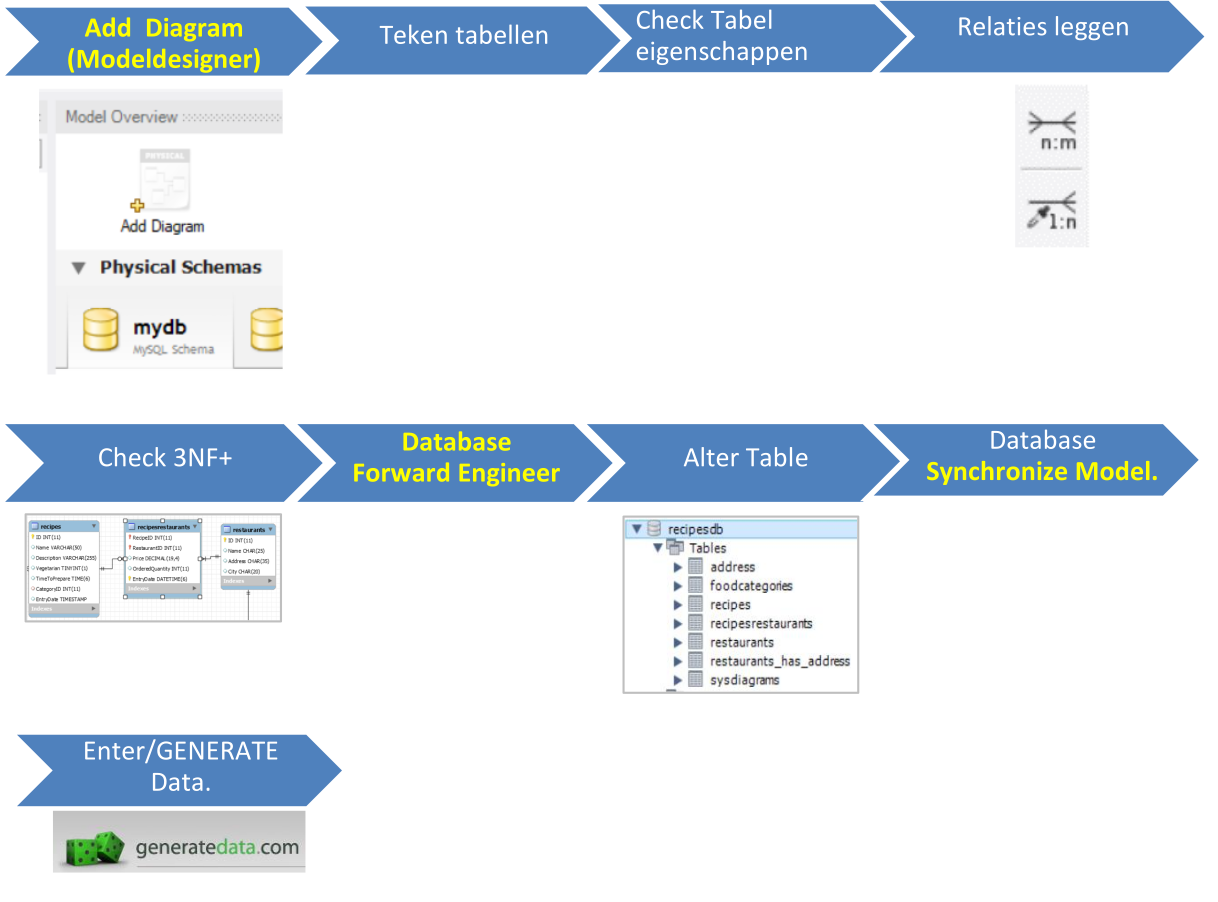
\includegraphics[width=0.8\textwidth]{overzicht-forward-engineering.png}
    \caption{Overzicht forward engineering}
\end{figure}

\subsection{Dump en Restore een schema/database in MySQL}
\subsubsection{Een dump maken van een schema/database}
Het bewaren van een MySQL database of schema vraagt twee acties:

\begin{itemize}
    \item Het opslaan van het aangemaakte diagram (*.mwb)
    \item Een dump maken van de database (*.sql). Een dump genereert het SQL-script om de database opnieuw aan te maken (restoren)
    \item In MySQL Workbench: Management Tab $\rightarrow$ Data Export
\end{itemize}

\subsubsection{Een database/schema restoren}
\begin{itemize}
    \item Uitvoeren van de dump (SQL-script), ofwel rechtstreeks in een query venster, ofwel via het menu item `Data Import'.
    \item Optioneel: een bewaard model (EERD) openen, of een model genereren via Home $\rightarrow$ Models menu $\rightarrow$ Create EER model from Database
\end{itemize}


\section{MySQL in de programmeeromgeving}

SQL-server data kan op verschillende manieren opgehaald en bewerkt worden (CRUD):
\begin{itemize}
    \item In een query venster (bv MySQL workbench)
    \item In een applicatieprogramma (bv Python)
    \item In programmablokken op SQL server: views, stored procedures, functies, triggers en events
\end{itemize}

\subsection{Programmablokken op MySQL server}

\subsubsection{Stored procedure}
Een stored procedure bevat IN en OUT parameters. Met de IN-parameters voert een stored
procedure een bewerking uit waarbij de OUT parameter(s) kunnen worden ingevuld. 

Typisch voert een procedure één of meerdere CRUD acties uit en voorziet hierbij een terugdraaimogelijkheid
voor foutief uitgevoerde transactie (= een transactie rollback).

\underline{Voorbeeld:} geld transfer, winkelkarretje opvullen.
\subsubsection{Function}

Een function voert ook bewerkingen uit op basis van IN parameters maar returnt altijd een
resultaat. Een stored procedure returnt geen resultaat (maar vult een parameter in).

\underline{Voorbeeld:} bij ingave van een product-ID krijg je naam, prijs maar ook de verkoopcijfers van de
maand van het product terug.

\subsubsection{Trigger}

Een trigger wordt geactiveerd door de SQL-server zelf als resultaat van een bepaalde actie.


\underline{Voorbeeld:} Wanneer en INSERT zijn gegevens gaat bewaren wordt een validatietrigger
(validatiecontrole) gestart. Enkel als de gegevens beantwoorden aan een reeks basisregels worden
de waarden bewaard. 

\underline{Voorbeeld:} Het verwittigen dat een klant te veel openstaande rekeningen heeft bij het plaatsen 
van zijn nieuw order.

\subsubsection{Event}

Ook een event wordt (zoals een trigger) geactiveerd door de server zelf. Een event wordt wel
geactiveerd op een bepaald tijdstip, terwijl trigger start op basis van een actie).

\underline{Voorbeeld:} Op het einde van de maand wordt automatisch een backup uitgegvoerd van alle
tabellen op de server

\subsection{Applicatienoden naast CRUD}
Wanneer je CRUDs onderbrengt in een applicatie is extra aandacht nodig voor volgende elementen:


\begin{itemize}
    \item Hoe en waar beveiligen. (=SECURITY = Authenticatie + autorisatie)?
    \item Hoe verhinderen dat hackers moedwillig schade aanbrengen (= VULNERABILITY = kwetsbaarheid)?
    \item Hoe automatisch onderhoudsacties (zoals backup) starten? (=PROGRAMABILITY)
    \item Hoe SQL fouten opsporen (applicatie fouten) met LOGGING mechanismen?
    \item Hoe verhinderen dat eenzelfde record op hetzelfde moment door meerdere personen aangepast wordt (=CONCURRENCY mechanisme).
    \item Hoe de database over verschillende servers (cloud) splitsen? Verticaal (= kolommen over servers spreiden) of horizontaal (=records over servers spreiden = sharding)?
    \item Hoe een transactie die dreigt mis te lopen terugdraaien (= TRANSACTIE ROLLBACK)?
    \item Hoe een falende database zo snel mogelijk weer online krijgen (=DATABASE RECOVERY)?
\end{itemize}

\subsection{Splitsen van verantwoordelijkheden}
Voor eenvoud van onderhoud en uibreidingen van code kiest men vaak om een server of een stukje code zijn eigen
verantwoordelijkheid te geven $\Rightarrow$ Single Point of Responsibility

\begin{figure}[H]
    \centering
    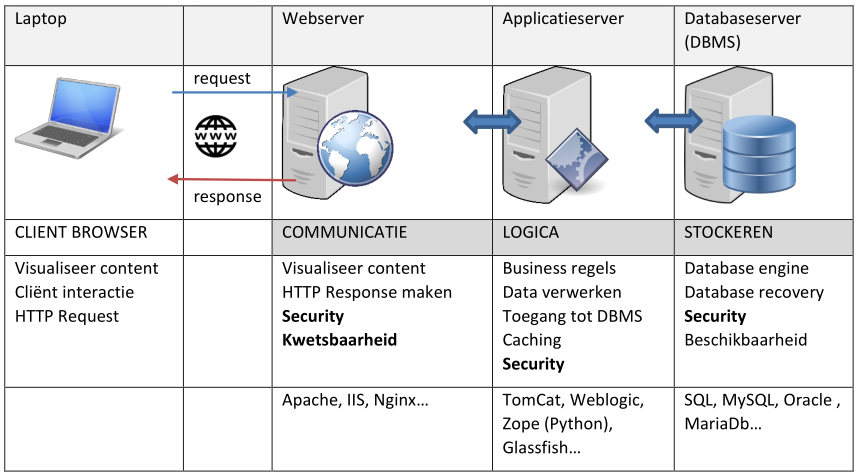
\includegraphics[width=0.9\textwidth]{Screenshot_20200429_135824.png}
    \caption{Splitsing van verantwoordelijkheid}
\end{figure}

\section{Applicatieprogramma in verschillende lagen (tiers)}
Net zoals de verschillende servers kan ook het applicatieprogramma opgesplitst worden in verschillende verantwoordeijkheden:

Applicatieprogramma = data access + logica + beveiliging:

\subsection{Data Access}
Een data-accessor tier of data-accessor laag verzamelt alle code die de toegang tot de database verzorgt. De
klasse of functie die connectie met de database maakt noemt men de connector. Zo is er een Python
connector voor MySQL, een C\# connector voor SQL enz...

\subsection{Logica}
De applicatie logica (ook business logica genoemd) verwerkt de data uit de databases en gebruikt hiervoor
berekeningen en afspraken zoals bijvoorbeeld kortingen en taxen bij distribiteur- of dealerprijzen.
Anderzijds zorgt validatie van input gegevens ervoor dat de gebruiker geen verkeerde data kan opvoeren
in de applicatie.

\subsubsection{Waar?}
Het aanbrengen van logica en het programma ervoor kan nu wel op verschillende plaatsen. Ga je de logica 
( vb. BTW berekenen) programmeren op de databaseserver (vb. in functions of stored procedures) of ga je 
dit doen in het applicatieprogramma ( C\#, Python... ). Of ga je beide combineren? Er is geen algemene 
regel.


\subsection{Beveiliging}
De beveiliging is terug te vinden in gebruikers accounts met specifieke rollen zoals een administrator, een
anonieme gebruiker., een super user De beveiliging regelt authenticatie (=wie ben je) en autorisatie (waar
heb je toegang toe).

\subsubsection{Waar de beveiliging aanbrengen?}
OVERAL! Authenticatie en authorisatie MOET zowel in het applicatieprogramma (vb. op de
webserver, op de applicatieserver) als op de database (op de database server) gebeuren.

Elke applicatie laag (of tier) MOET beveiligd worden.

\section{Applicatiebeveiliging}
\subsection{Beveiliging filosofie}
\begin{itemize}
    \item Security is nooit af maar blijft een “ongoing project”. 100\% security bestaat niet.
    \item Een veel gebruikte beveiligings fylosofie voor data is het \bold{CIA model:}
    \begin{itemize}
        \item \bold{Confidentiality}: geef alleen toegang aan de juiste/gekende gebruikers (verhinder anderen).
        \item \bold{Integrity}: ER model verhindert accidentele aanpassingen, data komt alleen van “verwachte” locaties. De data blijft correct, actueel en volledig.
        \item \bold{Availability}: maak data alleen beschikbaar wanneer ze verwacht wordt (vb op afgesproken momenten, na een geslaagde validatie)
    \end{itemize}

    \begin{figure}[H]
        \centering
        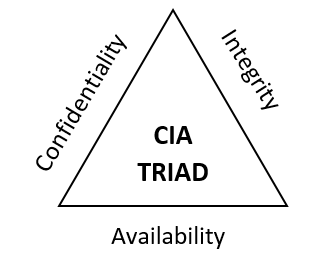
\includegraphics[width=0.2\textwidth]{ciamodel.png}
        \caption{CIA model}
    \end{figure}

    \item Beveiliging gebeurt op \bold{verschillende niveaus}. Voor elk niveau kan de diepte van beveiliging bepaald worden naar gelang belang, risico en budget

\end{itemize}

\subsubsection{Beveiligingsniveaus}
\bold{Fysisch}

\begin{itemize}
    \item Brandveilige ruimte
    \item Webserver met DMZ-faciliteiten (Demilitarized Zone): 2 verschillende fysische machines
\end{itemize}

\bold{Netwerk}

\begin{itemize}
    \item Plaats DBMS achter een firewall waarbij de firewall settings toegang filteren en routen
    \item Gebruik firewall configuratie tools om TCP poorten te configureren (poort 22 SSH, poort 80 http, poort 3306 MySQL ).
    \item Ontwerp de beveiliging alsof de firewall doorbroken is.
\end{itemize}

\bold{Operating system}

\begin{itemize}
    \item Onderhoud van de infrastructuur
    \item File toegang alleen voor bevoegden
    \item Hou software up-to-date (security patches)
\end{itemize}

\bold{Applicatie}

\begin{itemize}
    \item Website met authenticatie en authorisatie
    \item Website gewapend tegen kwetsbaarheid (XSS; CSRF)
    \item Accounts volgens het "least privileges": geef de gebruiker alleen wat hij nodig heeft volgens zijn rol of functie
    \item Installeer noch run onnodige services.
    \item Maak gebruik van rollen.
    \item Sterke wachtwoorden
    \item Disable root logins
    \item Remember "injection attacks"
    \item Hou mislukte aanmeldpogingen bij
    \item Gebruik een logboek
    \item Maak backups van data op een andere machine / ander netwerk
    \item Log files
    \item Gecommentarieerde code
\end{itemize}

\subsection{Principals met hun one-way passwoorden (hashed) en hun rollen}
Elke database bevat te beveiligen objecten. Permissies (of toegangcontroles) tot 
deze objecten worden toegekend aan een principal. Men gebruikt vaak het woord ``principal''
om ofwel één gebruiker ofwel een groep van gebruikers aan te duiden. 

Principals krijgen hiervoor \bold{``rollen''} toegekend. Door deze rollen krijgen principals 
``enkel'' toegang tot de zaken die ze nodig hebben (least-privileges).

\subsubsection{Server based principals in MSSQL = Administrative roles in MySQL}

Deze rollen zijn bedoeld voor administratie doeleinden binnen (My)SQL-server.
Logins kunnen toegekend worden aan een administrator (-rol) zonder dat hij een account moet hebben op één of meerdere databasen.

\subsubsection{Database based principals in MSSQL = Schema Privileges in MySQL}

Schema Privileges in MySQL bedoeld om gebruikers en hun bijhorende rollen aan te maken. 
De gebruikers krijgen een login, waarbij ze één of meerdere rollen toegewezen krijgen.

\subsection{De twee delen bij toegangscontrole:}

\begin{itemize}
    \item Authenticatie: Identificatie van de gebruiker en zijn rol (= identificeer de principal = WIE)
    \item Authorisatie: WAAR is de gebruiker toegelaten, waar zijn zijn rollen toegelaten
\end{itemize}

\subsubsection{Authenticatie}
Een login identificeert de principal en kan gebaseerd zijn op zowel Windows authenticatie (= gebruikersnaam bij
inloggen op windows) of SQL authenticatie (= login voor SQL) of voor beide. MSSQL voorziet default beide. MySQL
server verwacht default SQL-authenticatie maar beschikt over een plugin om dit te realiseren.

\subsubsection{Authorisatie}
Het SQL autorisatie model is gebaseerd op permissies die toegekend worden aan de twee eerder vermelde types
van principals: de \bold{server principal} en de \bold{database principal.}

Om de rechten te definiëren wordt gebruik gemaakt van schema’s en specifieke security tabellen of procedures. De
verantwoordelijken van deze schema’s, tabellen of procedures zijn opnieuw specifieke principals, die kunnen
aangepast worden in de tijd. Het default schema is \bold{dbo-schema}.

\underline{In MySQL:}

De authorisatiegegevens worden bijgehouden in een schema met naam ‘mysql.user’. Er wordt voor deze tabel
gebruik gemaakt van ``Account Management Statements''. Deze statements gebruiken kernwoorden zoals Create
USER, GRANT , REVOKE.

\section{Kwetsbaarheid (vulnerability) door SQL injectie}

Publieke toegang laat aan veel gebruikers (dus ook aan niet-ethische hackers) toe om via de
website toegang te krijgen. Men spreekt over de “kwetsbaarheid” (vulnerability) van de toepassing.

Een veel gebruikte techniek naar een applicatie toe is het injecteren van script (bvb. Javascript verborgen
in een image of in de headers van een webrequest, SQL injectie in statements die zichtbaar zijn in de
URL van de browser). Een dergelijke techniek op database niveau noemt men SQL-injectie.

\subsection{SQL injectie}

Hierbij worden kwaadwillige statements toegevoegd aan een input veld (of url) van een formulier.
Stel dat je bij een input veld, dat jouw naam verwacht, de woorden 'OR '1'='1 aan toevoegt.
Het 1=1 resulteert in een TRUE die de volledige OR functie altijd TRUE maakt.

In een C\# of Python applicatie werd de volgende SQL string opgebouwd:

\begin{lstlisting}[language=SQL]
SELECT * FROM Persons
WHERE LastName='''+ Johan'OR '1'=1 +"';
\end{lstlisting}

die na parsing op de database server resulteert in:

\begin{lstlisting}[language=SQL]
SELECT * FROM Persons
WHERE LastName= Johan OR '1' = '1';
\end{lstlisting}

Nog een voorbeeld van SQL injectie, die als resultaat een tabel verwijdert:

\begin{lstlisting}[language=SQL]
SELECT * FROM Persons
WHERE LastName='"Johan'; DROP TABLE Persons; --"';
\end{lstlisting}

Je verhindert SQL-injectie door op een correcte manier strings te formateren/escapen
of door het gebruik van parameters die zorgen voor de correcte formattering /escapen van input data op de web-
of applicatie-server. Expressies die gebruik maken van parameters noemt men ook ‘prepared statements’.

\section{DEMO DCL: authenticatie en authorisatie instellen}
Het toekennen en managen van permissies gebeurt met de SQL Data Control Language (DCL) statements. Je kan de
statements zelf schrijven of je kan ze laten aanmaken vanuit SSMS, de workbench.

\subsection{Beveiligen in MySQL met DCL}
Ref: \url{https://dev.mysql.com/doc/refman/8.0/en/security.html}

\subsubsection{Toevoegen van een gebruiker kan via T-SQL of via de workbench}

\begin{lstlisting}
CREATE USER 'recipesAdmin'@'localhost' IDENTIFIED BY 'recipesAdminPWD';

GRANT ALL privileges                    -- of SELECT, UPDATE ...
ON recipesDB                            -- niveau server, database, tabel, kolom
TO 'recipesAdmin'@'localhost'           -- de eerder aangemaakte gebruiker
WITH GRANT OPTION ;                     -- laat toe bevoegdheid door te geven

-- Controleer met een SELECT of de gebruiker nu bestaat in de table 'mysql.user':
SELECT * FROM mysql.user;
\end{lstlisting}

\subsubsection{Andere handige mysql instructies:}
\begin{lstlisting}
RENAME USER 'Johan' TO 'JohanV';
DROP USER 'Johan' @'localhost' ;
SET PASSWORD FOR 'Johan' = 'JohanPWD';
WITH MAX_QUERIES_PER_HOUR 2 -- GRANT aanvullen hiermee
REVOKE SELECT ON recipesDB TO -- REVOKE is de tegenhanger van GRANT
FLUSH privileges ; -- opkuisen van niet gebruikte privileges
\end{lstlisting}

\subsubsection{Privileges kunnen op verschillende niveaus worden gemaakt. }
Dit resulteert in verschillende keywoorden bij GRANT waarbij het wildcharacter * kan worden gebruikt

\url{https://dev.mysql.com/doc/refman/8.0/en/user-account-management.html}:

\begin{itemize}
    \item Gebruikers niveau voor alle databasen zou als volgt zijn: ON *.*
    \item Database niveau: ON recipesDB.*
    \item Tabel niveau : ON recipesDB.recipes
    \item Kolom niveau.
\end{itemize}

\bold{Oefeningen:}

\begin{itemize}
    \item Maak een gebruiker aan die enkel kan selecteren (SELECT) op de tabel recipes .
    \item Maak een tweede gebruiker die alle kolommen van recipes kan updaten en inserten.
\end{itemize}

\subsection{Beveiligen met MySQL workbench}

\subsubsection{Via het menu ``Users and Privilege''}
Je kan er een account selecteren, waarna je toegang tot login, beperkingen, rollen en privileges.Naast
standaard databases privileges , kan je bvb. ook privileges selecteren voor een typische administrator.

\subsubsection{Aanmaken van views en/of stored procedures voor één of meerdere gebruikers}

Je kan zover gaan dat een gebruiker enkel toegang heeft tot views en alleen bepaalde stored procedures kan uitvoeren.

\begin{itemize}
    \item Beveilig met T-SQL een view van je recipesDB zodat dit het enige is wat een reguliere gebruiker kan doen.

    \begin{lstlisting}[language=SQL]
    GRANT SELECT privileges ON eenRecipesView
    \end{lstlisting}

    \item Ken de procedures in recipesDB alleen toe aan de administrator. Een reguliere gebruiker kan ze
    niet zien noch gebruiken.

    \begin{lstlisting}[language=SQL]
    GRANT EXECUTE privileges ON eenProcedure
    \end{lstlisting}

\end{itemize}

\subsubsection{INFORMATION\_SCHEMA database}
MySQL maakt intern gebruik van een INFORMATION\_SCHEMA database. De privileges van gebruikers
worden ook hierin bewaard.

\url{https://dev.mysql.com/doc/refman/5.7/en/information-schema.html}

\subsubsection{Encrypteren van wachtwoorden}

MySQL Workbench voorziet default hashing. MySQL voorziet hiervoor een aantal encryptfuncties voor one way hashing (= er is
geen decrypt): SHA, SHA(1), SHA2. Deze laatste (SHA2) verwacht wel SSL support voor de connectie.

Bij one way hashing moet een paswoord dat opgevoerd wordt in de applicatie (Python, PHP) eerst
geëncrypteerd worden. Het geëncrypteerde resultaat wordt verstuurd en vergeleken met de hash in de
database.

\subsubsection{Plugins}

MySQL voorziet verschillende plugins, die je kan installeren via het Scripting menu van de Workbench of via T-SQL

Overzicht plugins: \url{https://dev.mysql.com/doc/refman/8.0/en/plugin-types.html}

\section{Transacties}
Een transactie is een reeks bewerkingen die op de database worden uitgevoerd.
Men noemt het ook \bold{Logical Units Of Work (LUW)}. De term ``logical units'' wijst erop dat een
reeks van verschillende bewerkingen \bold{ofwel succesvol of helemaal niet} worden uitgevoerd.

Wanneer al die acties van elkaar afhangen, spreekt men van een ``atomaire''
transactie omdat ze als één geheel moeten worden uitgevoerd. Ze hangen als het ware samen zoals een atoom, dat
niet kan bestaan zonder zijn electronen of protonen.

\subsection{Atomaire transacties}

Om fouten te vermijden werkt men bij atomaire transacties met een ``START Transaction'', die ofwel succesvol
eindigt (=COMMIT transaction) ofwel in zijn totaliteit niet uitgevoerd wordt. Bij een niet geslaagde atomaire
transacties worden de reeds uitgevoerde bewerkingen teruggedraaid in de tijd (=ROLLBACK transaction)


\subsubsection{Rollback vanuit een stored procedure}

Dit transactie mechanisme wordt vooral toegepast in een procedure (stored pocedure). Dit betekent dat het nodig
wordt om te monitoren of een fout zich voordoet tijdens de uitvoer van deze procedure. Bij een fout gebeurt
ROLLBACK, anders een COMMIT.

\subsubsection{Fouten monitoren in een procedure of in het applicatieprogramma (python).}

Het transactie mechanisme kan evengoed uitgevoerd worden in het applicatieprogramma. Je maakt in het
applicatieprogramma gebruik van een try/catch. Bij een error vangt de catch de fout op en zorgt deze catch voor de
rollback. Zonder error wordt de commit uitgevoerd.

\subsection{Concurrent transacties.}

Met concurrency verwijst men naar acties die simultaan gebeuren. Hoe ga je om met twee bewerkingen (door
bijvoorbeeld twee gebruikers) die eenzelfde rij of record willen aanpassen. Als ontwikkelaar kan je het concurrency
gedrag definiëren. 

Concurrency gedrag kan door een 3-tal elementen ingesteld worden: een transactie isolatie
niveau, een locking mechanisme en cursor concurrency (= laatste specifiek voor MSSQL)

\subsubsection{Transactie isolatie niveau:}
De volgende leesproblemen kunnen voorkomen wanneer verschillende transacties op eenzelfde resource
data gaan aanpassen:

\begin{itemize}
    \item \bold{Dirty Read}: Bij herlezen worden wijzigingen die nog niet gecommit zijn gedetecteerd op de zopas ingevoerde data.
    \item \bold{Nonrepeatable Read}: Bij herlezen worden wijzigingen gedetecteerd doordat intussen commits wel uitgevoerd werden.
    \item \bold{Phantom Read}: Bij herlezen zijn nieuwe data, nieuwe rijen toegevoegd door een commited transactie.
\end{itemize}

Om dit te verhinderen bestaan verschillende \bold{isolatieniveaus}. Het isolatie niveau geeft aan in welke mate de
gebruikers van elkaar geïsoleerd zijn. Een isolatieniveau kan gaan van Read Uncommited tot Serializable (zie
referentie).

Zo blokkeert REPEATABLE READ alle rijen die op een bepaald ogenblijk gelezen worden, waardoor ze niet kunnen
gewijzigd worden door derden. Dit is de default instelling bij het InnoDB engine. De instelling kan wel aangepast
worden.

\begin{lstlisting}[language=SQL]
SET TRANSACTION ISOLATION LEVEL REPEATABLE READ
\end{lstlisting}

De term SERIALIZABLE transactie verwijst dan weer naar SQL instructies die zonder probleem in een willekeurige
volgorde na elkaar of naast elkaar kunnen worden gebruikt.
Een isolatie niveau SERIALIZABLE vertegenwoordigt de hoogste isolatie graad.

\subsubsection{Locking mechanismes voor instructies}
Bij locking definieert men hoe een instructie een resource blokkeert t.o.v. een andere instructie. 
De duurtijd van een blokkade duurt nooit langer dan de duurtijd van de transactie. Verschillende types resources kunnen
geblokkeerd worden. Men spreekt over de ``granulariteit'' van een lock. Zo kan locken op database niveau, op tabel
niveau, op rij niveau.

Let wel: hoe meer je locking toepast, hoe lager het concurrency niveau wordt. Zo kan door intensief locken een
\bold{``deadlock''} ontstaan. Bij een deadlock wachten verschillende gebruikers op elkaar tot een rij of tabel vrij gegeven
wordt. Gebeurt dit niet dan zorgt een timeout voor een rollback. Een deadlock kan vermeden worden door voor een
SQL instructie alle benodigde bronnen bij het begin van de transactie te locken.

\subsubsection{Cursor concurrency}

Met cursor-concurrency kunnen verschillende cursor types (optimistisch; pessimistisch) ingesteld worden. De cursor
is een pointer die het resultaat set van een transactie overloopt en beheert. De cursor concurrency instelling wordt
gebruikt binnen MSSQL.

\bold{Optimistic Concurrency}

Optimistic concurrency gaat ervan uit dat er weinig kans is op concurrency problemen. Gegevens
worden ingelezen, de transactie (die kan atomair zijn) wordt verwerkt, wijzigingen worden
uitgevoerd en op het einde gebeurt een controle (heruitlezen) om te zien of er geen conflict was.

\bold{Pessimistic Concurrency}

Pessimistic concurrency gaat ervan uit dat er juist wel een conflict zal optreden en worden daarom
eerst de locks aangebracht bij de eerste opdracht van een transactie. Pas bij het einde van de
transactie wordt de LOCK vrijgegeven.


\section{Logfiles}

Logfiles zijn vooral van belang in een productie omgeving voor opsporen van recursieve of sporadische fouten,
gekend onder de noemer “error-handling”.

\subsection{Logfiles in MySQL}

MySQL kan verschillende logs genereren. Elke log heeft een verschillend doel en kan aan- of afgezet worden via de
server option file. De logfiles zijn standaard txt files.

\begin{itemize}
\item \underline{Error log (*.err file):} bijhouden van fouten en exceptions
\item \underline{General query log (*.log file):} bijhouden wanneer een gebruiker aanlogt, disconnecteert en welke queries aangevraagd werden. Deze log kan een beeld geven over de activiteit (trafiek) van jouw server.
\item \underline{Slow query log ( *-slow.log file):} bijhouden van queries die te lang duren. De duurtijd is via de optie long- query-time instelbaar en staat default op 10sec.
\item \underline{Binary log (instellen via log-bin optie):} bijhouden van aanpassingen die door de server zelf geïnitieerd werden. Dit speelt een rol bij backup en recovery van files.
\end{itemize}

Wanneer de files te groot worden kunnen ze verwijderd worden op een bepaalde leeftijd (Logfile expiration) of
wordt een logfile rotation techniek gebruikt. Deze laatste herbenoemt of overschrijft één of meerdere logfiles.

Error handling in MySQL gebeurt hoofdzakelijk via zijn programmeer mogelijkheden. Een try/catch is niet
beschikbaar binnen MySQL. In plaats daarvan wordt een handler gedefinieerd. Deze handler kan reageren op alle
exceptions of specifieke foutcodes. Deze foutcodes worden opgesomd in de referentie en zijn een getal tussen 1000
en 3227. De handler kan zorgen voor een specifieke foutboodschap, voor een rollback, of voert een willekeurige SQL-
instructie uit.

\section{Database recovery}

Databasen en servers kunnen falen en toch moet zo snel mogelijk de server weer online komen met liefst geen
dataverlies. Dit is database-recovery. Recovery wordt gerealiseerd via reprocessing of via rollback/rollforward.

\subsection{Reprocessing}
Reprocessing verwacht het regelmatig backuppen van de database, zodat de backup na faling onmiddellijk
kan gerestored worden. Transacties die gebeurden tijdens de crash zijn natuurlijk niet geregistreerd.
Gevolg: reprocessing is niet bruikbaar bij bankverrichtingen, vliegtuigreservaties...


\subsection{Rollback/rollforward}
Rollback/Rollforward verwachten dat na elke save ook alle erna komende transacties gestockeerd worden
in een log bestand (= een kopie bijhouden met alle datawijzigingen in chronische volgorde. START als
keywoord om het begin van een transactie aan te duiden en COMMIT om het resultaat weer te geven.).

\begin{itemize}
    \item Rollforward: na restore worden alle gestockeerde transacties opnieuw uitgevoerd. Ze worden opgehaald uit de save en heruitgevoerd.
    \item Rollback: verwijdert de mislukte transacties op het moment van de crash en herstart de geldige transacties, die in bewerking waren tijdens de storing.
\end{itemize}

Een rollback/rollforward wordt vaak met een try/catch gecombineerd. Als de try mislukt wordt dit opgevangen in de
catch, die zorgt voor een rollback (zie bij error logging)

Als administrator van een database zal je wel meest geïnteresseerd zijn in het reprocessen van de volledige server
en zijn databasen. Om dit te automatiseren zal een dump via code (via een trigger, procedure of script) nodig zijn.


\end{document}